%%% Hlavní soubor. Zde se definují základní parametry a odkazuje se na ostatní části. %%%

%% Verze pro jednostranný tisk:
% Okraje: levý 40mm, pravý 25mm, horní a dolní 25mm
% (ale pozor, LaTeX si sám přidává 1in)
\documentclass[12pt,a4paper]{report}
\setlength\textwidth{145mm}
\setlength\textheight{247mm}
\setlength\oddsidemargin{15mm}
\setlength\evensidemargin{15mm}
\setlength\topmargin{0mm}
\setlength\headsep{0mm}
\setlength\headheight{0mm}
% \openright zařídí, aby následující text začínal na pravé straně knihy
\let\openright=\clearpage

%% Pokud tiskneme oboustranně:
% \documentclass[12pt,a4paper,twoside,openright]{report}
% \setlength\textwidth{145mm}
% \setlength\textheight{247mm}
% \setlength\oddsidemargin{14.2mm}
% \setlength\evensidemargin{0mm}
% \setlength\topmargin{0mm}
% \setlength\headsep{0mm}
% \setlength\headheight{0mm}
% \let\openright=\cleardoublepage

%% Vytváříme PDF/A-2u
\usepackage[a-2u]{pdfx}

%% Přepneme na českou sazbu a fonty Latin Modern
\usepackage[slovak]{babel}
\usepackage{lmodern}
\usepackage[T1]{fontenc}
\usepackage{textcomp}

%% Použité kódování znaků: obvykle latin2, cp1250 nebo utf8:
\usepackage[utf8]{inputenc}

%%% Další užitečné balíčky (jsou součástí běžných distribucí LaTeXu)
\usepackage{amsmath}        % rozšíření pro sazbu matematiky
\usepackage{amsfonts}       % matematické fonty
\usepackage{amsthm}         % sazba vět, definic apod.
\usepackage{bbding}         % balíček s nejrůznějšími symboly
			    % (čtverečky, hvězdičky, tužtičky, nůžtičky, ...)
\usepackage{bm}             % tučné symboly (příkaz \bm)
\usepackage{graphicx}       % vkládání obrázků
\usepackage{fancyvrb}       % vylepšené prostředí pro strojové písmo
\usepackage{indentfirst}    % zavede odsazení 1. odstavce kapitoly
\usepackage{natbib}         % zajištuje možnost odkazovat na literaturu
			    % stylem AUTOR (ROK), resp. AUTOR [ČÍSLO]
\usepackage[nottoc]{tocbibind} % zajistí přidání seznamu literatury,
                            % obrázků a tabulek do obsahu
\usepackage{icomma}         % inteligetní čárka v matematickém módu
\usepackage{dcolumn}        % lepší zarovnání sloupců v tabulkách
\usepackage{booktabs}       % lepší vodorovné linky v tabulkách
\usepackage{paralist}       % lepší enumerate a itemize
\usepackage{xcolor}         % barevná sazba

% dodané mimo šablonu
\usepackage{graphicx}		% umisti obrazky vedle sebe
\usepackage{subcaption}		% umisti obrazky vedle sebe
\usepackage{enumitem}
\usepackage{dirtree}		% pro strom adresářů příloh
\usepackage{hyperref}
%\usepackage[cache=false]{minted}			% syntax highlight
%\usepackage{algpseudocode}  
%\usepackage{algorithm}
\usepackage{multicol}

\usepackage[shortcuts]{extdash}		% pro možnost zakázání dělení slov kolem pomlčky
									% např. pro slovo "chce-li", které lze zapsat "che\=/li"

%%% Údaje o práci

% Název práce v jazyce práce (přesně podle zadání)
\def\NazevPrace{Analyzátor USB paketov}

% Název práce v angličtině
\def\NazevPraceEN{USB Packet Analyzer}

% Jméno autora
\def\AutorPrace{Peter Lakatoš}

% Rok odevzdání
\def\RokOdevzdani{2021}

% Název katedry nebo ústavu, kde byla práce oficiálně zadána
% (dle Organizační struktury MFF UK, případně plný název pracoviště mimo MFF)
\def\Katedra{Katedra distribuovaných a~spolehlivých systémů}
\def\KatedraEN{Department of~Distributed and~Dependable Systems}

% Jedná se o katedru (department) nebo o ústav (institute)?
\def\TypPracoviste{Katedra}
\def\TypPracovisteEN{Department}

% Vedoucí práce: Jméno a příjmení s~tituly
\def\Vedouci{Mgr.~Pavel Ježek,~Ph.D.}

% Pracoviště vedoucího (opět dle Organizační struktury MFF)
\def\KatedraVedouciho{Katedra distribuovaných a~spolehlivých systémů}
\def\KatedraVedoucihoEN{Department of~Distributed and~Dependable Systems}

% Studijní program a obor
\def\StudijniProgram{Informatika}
\def\StudijniObor{Programování a~softwarové systémy}

% Nepovinné poděkování (vedoucímu práce, konzultantovi, tomu, kdo
% zapůjčil software, literaturu apod.)
\def\Podekovani{%
Týmto by som chcel poďakovať svojmu vedúcemu Mgr.~Pavlovi Ježekovi,~Ph.D., za jeho čas, ochotu, cenné rady a nápady bez ktorých by táto práca nemohla vzniknúť. Veľká vďaka patrí zároveň mojej rodine a priateľom za ich podporu počas celého môjho štúdia.
}

% Abstrakt (doporučený rozsah cca 80-200 slov; nejedná se o zadání práce)
\def\Abstrakt{%
USB zbernica je dnes jedným z najrozšírenejších spôsobov pripojenia periférií k~počítaču. 
Cieľom práce bolo vytvoriť software, ktorý analyzuje zachytenú komunikáciu medzi zariadnením pripojeným na~danú zbernicu a~počítačom.

Aplikácia prehľadným spôsobom vizuálne zobrazuje zanalyzované dáta -- konkrétne sa zameriava na~HID triedu zariadení a~ponúka aj sémantický význam jej úzkej podmnožiny do~ktorej patria myš, klávesnica a~joystick. Pri vizuálnej reprezentácii dát sa práca inšpiruje rôznymi dostupnými softwarmi, pričom rozlične kombinuje resp. dopĺňa ich vlastnosti a~implementuje z~nich tie, ktoré vníma ako najlepšie riešenie v danej situácii.

Dôležitá vlastnosť aplikácie je parsovanie HID Report Descriptoru vďaka ktorému bude v budúcnosti jednoduchšie pridať sémantickú analýzu rôznym ďalším HID zariadeniam. Celkový návrh aplikácie by mal ponúknuť možnosť budúcej implementácie ďalších USB tried pre~prípadné rozšírenie.
}
\def\AbstraktEN{%
The USB bus is the most common way of connecting peripherals to personal computers. The goal of this thesis is to create an application which analyzes communication between a device connected to this bus and a computer.

The application is capable to readably display analyzed data, with specific focus on HID class devices. The application implements semantic analysis of a subset of HID devices consisting of mice, keyboards and joysticks. The methods that the application uses to visually represent data are inspired by already existing applications, where our application combines them and impoves their capabilities to achieve better results.

Notable part of the application is its ability to parse HID Report Descriptor, to accomplish easier addition of new HID devices for semantic analysis. Overall design of the application is general enough to allow simple addition of analysis for other USB classes.
}

% 3 až 5 klíčových slov (doporučeno), každé uzavřeno ve složených závorkách
\def\KlicovaSlova{%
{USB} {HID} {Analyzátor}
}
\def\KlicovaSlovaEN{%
{USB} {HID} {Analyzer}
}

%% Balíček hyperref, kterým jdou vyrábět klikací odkazy v PDF,
%% ale hlavně ho používáme k uložení metadat do PDF (včetně obsahu).
%% Většinu nastavítek přednastaví balíček pdfx.
\hypersetup{unicode}
\hypersetup{breaklinks=true}

%% Definice různých užitečných maker (viz popis uvnitř souboru)
%%% Tento soubor obsahuje definice různých užitečných maker a prostředí %%%
%%% Další makra připisujte sem, ať nepřekáží v ostatních souborech.     %%%

%%% Drobné úpravy stylu

% Tato makra přesvědčují mírně ošklivým trikem LaTeX, aby hlavičky kapitol
% sázel příčetněji a nevynechával nad nimi spoustu místa. Směle ignorujte.
\makeatletter
\def\@makechapterhead#1{
  {\parindent \z@ \raggedright \normalfont
   \Huge\bfseries \thechapter. #1
   \par\nobreak
   \vskip 20\p@
}}
\def\@makeschapterhead#1{
  {\parindent \z@ \raggedright \normalfont
   \Huge\bfseries #1
   \par\nobreak
   \vskip 20\p@
}}
\makeatother

% Toto makro definuje kapitolu, která není očíslovaná, ale je uvedena v obsahu.
\def\chapwithtoc#1{
\chapter*{#1}
\addcontentsline{toc}{chapter}{#1}
}

% Trochu volnější nastavení dělení slov, než je default.
\lefthyphenmin=2
\righthyphenmin=2

% Zapne černé "slimáky" na koncích řádků, které přetekly, abychom si
% jich lépe všimli.
\overfullrule=1mm

%%% Makra pro definice, věty, tvrzení, příklady, ... (vyžaduje baliček amsthm)

\theoremstyle{plain}
\newtheorem{veta}{Věta}
\newtheorem{lemma}[veta]{Lemma}
\newtheorem{tvrz}[veta]{Tvrzení}

\theoremstyle{plain}
\newtheorem{definice}{Definice}

\theoremstyle{remark}
\newtheorem*{dusl}{Důsledek}
\newtheorem*{pozn}{Poznámka}
\newtheorem*{prikl}{Příklad}

%%% Prostředí pro důkazy

\newenvironment{dukaz}{
  \par\medskip\noindent
  \textit{Důkaz}.
}{
\newline
\rightline{$\qedsymbol$}
}

%%% Prostředí pro sazbu kódu, případně vstupu/výstupu počítačových
%%% programů. (Vyžaduje balíček fancyvrb -- fancy verbatim.)

\DefineVerbatimEnvironment{code}{Verbatim}{fontsize=\small, frame=single}

%%% Prostor reálných, resp. přirozených čísel
\newcommand{\R}{\mathbb{R}}
\newcommand{\N}{\mathbb{N}}

%%% Užitečné operátory pro statistiku a pravděpodobnost
\DeclareMathOperator{\pr}{\textsf{P}}
\DeclareMathOperator{\E}{\textsf{E}\,}
\DeclareMathOperator{\var}{\textrm{var}}
\DeclareMathOperator{\sd}{\textrm{sd}}

%%% Příkaz pro transpozici vektoru/matice
\newcommand{\T}[1]{#1^\top}

%%% Vychytávky pro matematiku
\newcommand{\goto}{\rightarrow}
\newcommand{\gotop}{\stackrel{P}{\longrightarrow}}
\newcommand{\maon}[1]{o(n^{#1})}
\newcommand{\abs}[1]{\left|{#1}\right|}
\newcommand{\dint}{\int_0^\tau\!\!\int_0^\tau}
\newcommand{\isqr}[1]{\frac{1}{\sqrt{#1}}}

%%% Vychytávky pro tabulky
\newcommand{\pulrad}[1]{\raisebox{1.5ex}[0pt]{#1}}
\newcommand{\mc}[1]{\multicolumn{1}{c}{#1}}


%% Titulní strana a různé povinné informační strany
\begin{document}
%%% Titulní strana práce a další povinné informační strany

%%% Titulní strana práce

\pagestyle{empty}
\hypersetup{pageanchor=false}

\begin{center}

\centerline{\mbox{
\includegraphics[width=166mm]{img/logo-cs.pdf}}}

\vspace{-8mm}
\vfill

{\bf\Large BAKALÁŘSKÁ PRÁCE}

\vfill

{\LARGE\AutorPrace}

\vspace{15mm} 

{\LARGE\bfseries\NazevPrace}

\vfill

\Katedra

\vfill

{
\centerline{\vbox{\halign{\hbox to 0.45\hsize{\hfil #}&\hskip 0.5em\parbox[t]{0.45\hsize}{\raggedright #}\cr
Vedoucí bakalářské práce:&\Vedouci \cr
\noalign{\vspace{2mm}}
Studijní program:&\StudijniProgram \cr
\noalign{\vspace{2mm}}
Studijní obor:&\StudijniObor \cr
}}}}

\vfill

% Zde doplňte rok
Praha \RokOdevzdani

\end{center}

\newpage

%%% Následuje vevázaný list -- kopie podepsaného "Zadání bakalářské práce".
%%% Toto zadání NENÍ součástí elektronické verze práce, nescanovat.

%%% Strana s čestným prohlášením k bakalářské práci

\openright
\hypersetup{pageanchor=true}
\pagestyle{plain}
\pagenumbering{roman}
\vglue 0pt plus 1fill

\noindent
Prohlašuji, že jsem tuto bakalářskou práci vypracoval(a) samostatně a výhradně
s~použitím citovaných pramenů, literatury a dalších odborných zdrojů.
Tato práce nebyla využita k získání jiného nebo stejného titulu.

\medskip\noindent
Beru na~vědomí, že se na moji práci vztahují práva a povinnosti vyplývající
ze zákona č. 121/2000 Sb., autorského zákona v~platném znění, zejména skutečnost,
že Univerzita Karlova má právo na~uzavření licenční smlouvy o~užití této
práce jako školního díla podle §60 odst. 1 autorského zákona.

\vspace{10mm}

\hbox{\hbox to 0.5\hsize{%
V \hbox to 6em{\dotfill} dne \hbox to 6em{\dotfill}
\hss}\hbox to 0.5\hsize{\dotfill\quad}}
\smallskip
\hbox{\hbox to 0.5\hsize{}\hbox to 0.5\hsize{\hfil Podpis autora\hfil}}

\vspace{20mm}
\newpage

%%% Poděkování

\openright

\noindent
\Podekovani

\newpage

%%% Povinná informační strana bakalářské práce

\openright

\vbox to 0.5\vsize{
\setlength\parindent{0mm}
\setlength\parskip{5mm}

Název práce:
\NazevPrace

Autor:
\AutorPrace

\TypPracoviste:
\Katedra

Vedoucí bakalářské práce:
\Vedouci, \KatedraVedouciho

Abstrakt:
\Abstrakt

Klíčová slova:
\KlicovaSlova

\vss}
\newpage \openright %\nobreak
\vbox to 0.49\vsize{
\setlength\parindent{0mm}
\setlength\parskip{5mm}

Title:
\NazevPraceEN

Author:
\AutorPrace

\TypPracovisteEN:
\KatedraEN

Supervisor:
\Vedouci, \KatedraVedoucihoEN

Abstract:
\AbstraktEN

Keywords:
\KlicovaSlovaEN

\vss}

\newpage

\openright
\pagestyle{plain}
\pagenumbering{arabic}
\setcounter{page}{1}


%%% Strana s automaticky generovaným obsahem bakalářské práce

\tableofcontents

%%% Jednotlivé kapitoly práce jsou pro přehlednost uloženy v samostatných souborech
\chapter{Úvod}

USB je najrozšírenejšia zbernica na pripojenie rôznych periférií k počítaču. Vznikla v druhej polovici 90. rokov 20. storočia, kedy boli rôzne zariadenia a ich porty veľmi úzko mapované. Na pripojenie základných zariadení ako myš alebo klávesnica slúžil napríklad sériový port PS/2~\cite{ps2_port}. K pripojeniu tlačiarne sa často používal paralelný port Centronics~\cite{parallel_port}. Ešte pred PS/2 portom sa myš pripájala cez veľmi známy sériový port RS-232~\cite{rs232_port}. Všetky tieto porty boli typu \textit{point-to-point} -- na jeden port je možné pripojiť len jedno zariadenie. Toto sa paralelným portom dalo čiastočné obísť tým, že niektoré zariadenia podporovali tzv. \textit{daisy chain} -- do pripojeného zariadenia sa pripojí ďalšie zariadenie, do toho sa pripojí ďalšie, atď. (napríklad typická tlačiareň toto nepodporovala, takže musela byť pripojená na konci \textit{daisy chainu}). Existovala takisto paralelná \textit{SCSI} zbernica~\cite{scsi_hub}, ktorej návrh bol prispôsobený aby podporoval  \textit{daisy chain}. Tá fungovala dobre na zariadeniach ako externé HDD a skenery, ale bola nepraktická pre zariadenia ako myš a klávesnica.

USB vzniklo za účelom nahradiť a zjednotiť tieto spôsoby pripojenia bežných periférií k počítaču. Návrh zbernice je založený na hviezdicovej topológii, ktorá umožňuje cez jeden port pripojiť až 127 zariadení súčasne. Z toho vyplýva, že USB interface v sebe zahŕňa obrovskú množinu protokolov, ktoré sú hierarchicky usporiadané. K analýze paketov ktoré sa pohybujú na danej zbernici nám slúžia tzv. USB paket analyzátory. Tie môžu mať podobu hardwarového zariadenia, alebo softwarovej aplikácie. Môžu slúžiť napríklad ako učebná pomôcka pre účel lepšieho pochopenia jednotlivých protokolov. Takisto sa často využívajú pri implementácii vlastného USB zariadenia na ladenie komunikácie medzi daným zariadením a driverom. Využitie ale majú aj v opačnom prípade, keď implementujeme vlastný driver a potrebujeme sledovať jeho komunikáciu s konkrétnym zariadením. Cieľom tejto práce bude naprogramovať funkčný softwarový USB analyzátor, ktorý by mal presnejšie slúžiť práve ako učebná pomôcka pre lepšie pochopenie určitej množiny protokolov. Cieľová platforma aplikácie bude Windows.

\section{Základné pojmy}

V tejto sekcii si vysvetlíme niektoré základné pojmy ktoré budeme neskôr v~texte používať.

\begin{figure}[!htb]
	\centering
	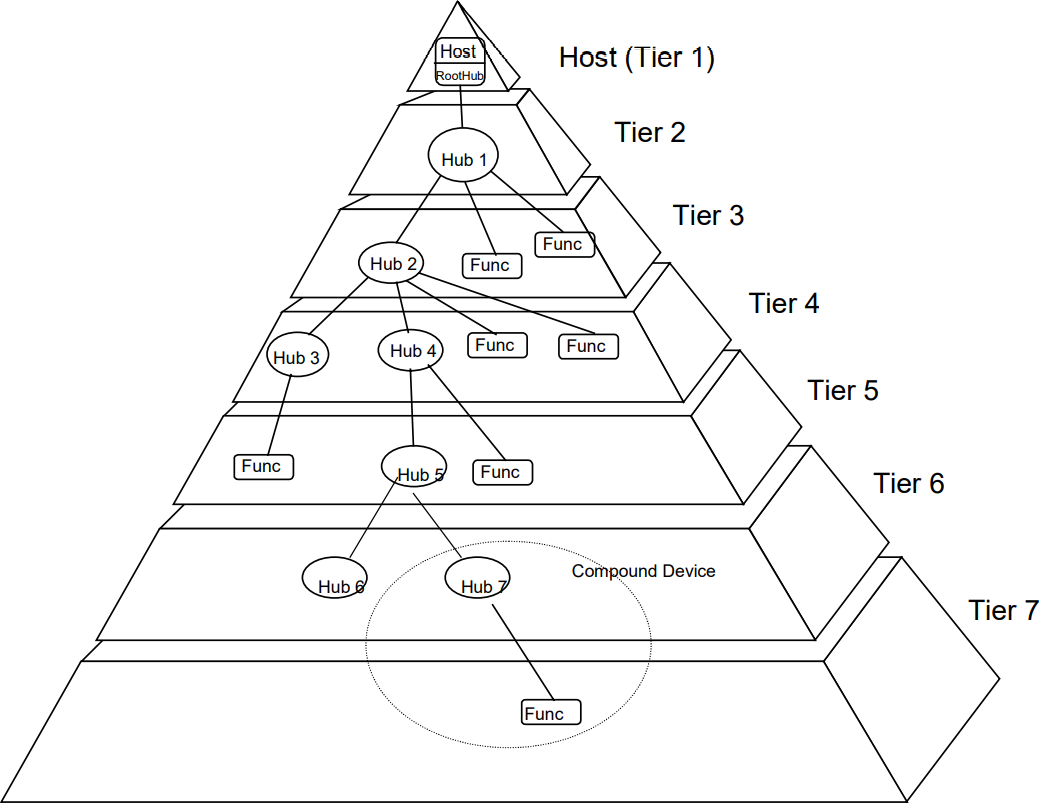
\includegraphics[width=\textwidth]{img/uvod_usb_topology}
	\caption{USB topológia. Obrázok prevzatý z USB 2.0 špecifikácie~\cite{usb_topology}.}
	\label{obr:uvod:usb_topology}
\end{figure}

Ako sme už vyššie spomínali a ako ilustruje obrázok~\ref{obr:uvod:usb_topology}, USB zbernica je založená na vrstevnatej hviezdicovej topológii. Na vrchu všetkého sa nachádza \textbf{USB Host}~\cite{usb_host} čo je systém do ktorého sa pripájajú ostatné USB zariadenia (v našom prípade je \textit{USB Host} počítač). \textbf{USB zariadenie}~\cite{usb_device} je buď:
\begin{itemize}
\item \textbf{Hub}~\cite{usb_hub} -- poskytuje dodatočné pripojenia k USB zbernici.
\item \textbf{Funkcia}~\cite{usb_function} -- poskytuje novú funkcionalitu systému (napríklad joystick, reproduktory, myš a pod.)
\end{itemize}

 V každom USB systéme sa nachádza práve jeden \textit{USB Host}. Ten má integrovaný tzv. \textbf{Root Hub}~\cite{usb_host}, ktorý poskytuje možné body pripojenia pre ďalšie zariadenia. Interface medzi hostom a USB sa nazýva \textbf{Host Controller}~\cite{usb_host}. Vzhľadom na niektoré časové obmedzenia USB je maximálny počet vrstiev 7 (vrátane \textit{USB Host} vrstvy). Každý káblový segment je \textit{point-to-point}~\cite{usb_bus_topology} spojenie medzi:
\begin{itemize}
\item \textit{host} $\longleftrightarrow$ \textit{hub}/\textit{funkcia}
\item \textit{hub} $\longleftrightarrow$ \textit{hub}/\textit{funkcia}
\end{itemize}

USB zariadenia využívajú tzv. \textbf{descriptory} na predávanie informácií o sebe samých. \textbf{Descriptor}~\cite{usb_descriptor} je dátová štruktúra s predom definovaným formátom. Existuje viacero typov \textit{USB descriptorov} (device, endpoint, interface atď.), ktorých význam si vysvetlíme neskôr.

Vzhľadom na hierarchickú štruktúru USB protokolov sa \textit{USB zariadenia} delia na rôzne triedy~\cite{usb_classes}. USB trieda je zoskupenie zariadení (alebo interfacov) ktoré majú spoločné vlastnosti alebo funkcionalitu. Tieto triedy umožňujú USB hostovi identifikovať dané zariadenie a jeho funkcionalitu. Každá trieda má svoju vlastnú \textit{Class Specification} -- definuje správanie zariadení v jednotlivých triedach a opisuje ich komunikačný protokol, ktorý sa naprieč triedami líši. Takisto definuje rôzne descriptory, ktoré sú špecifické pre danú triedu. Príklady USB tried a jednotlivých zariadení ktoré do nich patria sú:
\begin{itemize}
\item Mass Storage (napr. SD karta a flash disk)
\item Audio (napr. reproduktory a slúchadlá)
\item HID -- Human Interface Device (napr. myš, klávesnica alebo joystick)
\end{itemize}

\textbf{Paket}~\cite{usb_packet} je súbor dát zoskupený na prenos po zbernici. Typicky sa skladá z troch častí:
\begin{itemize}
\item základné informácie o danom pakete (napríklad zdroj, cieľ, dĺžka) -- takisto nazývané hlavička paketu
\item samotné dáta
\item detekcia chýb, opravné bity
\end{itemize}

Komunikácia na zbernici medzi \textit{USB hostom} a \textit{zariadením} prebieha práve pomocou prenosu \textit{USB paketov}.   Existujú 4 typy takýchto prenosov~\cite{usb_type_transfers}:
\begin{itemize}
\item \textbf{Control Transfer} -- používa sa na nakonfigurovanie USB zariadenia v momente keď sa pripojí na zbernicu.
\item \textbf{Bulk Data Transfer} -- typicky pozostáva z väčšieho množstva dát ktoré sú posielané nárazovo (využívajú ho najmä tlačiarne alebo skener). Vďaka detekcii chýb na hardwarovej úrovni je zaistená správnosť prenesených dát.
\item \textbf{Interrupt Data Transfer} -- spoľahlivý prenos ktorý sa využíva hlavne na odovzdávanie aktuálnych informácií (ako napríklad pohyb myšou). Tieto informácie musia byť doručené USB zbernicou za čas kratší ako má špecifikované dané zariadenie.
\item \textbf{Isochronous Data Transfer} -- takisto nazývaný ako streaming v reálnom čase. Typický príklad je prenos zvuku.
\end{itemize}

Našu aplikáciu by sme chceli zamerať na Windows a tak si vysvetlíme ešte zopár špecifických pojmov, ktoré sa viažu na túto kokrétnu platformu.

Podľa MSDN dokumentácie~\cite{usbclientdriver} je \textbf{USB client driver} software nainštalovaný na počítači, ktorý komunikuje s USB zariadením aby spojazdnil jeho funkcionalitu. Žiaden \textit{USB client driver} ale nemôže priamo komunikovať so svojím zariadením. Namiesto toho vytvorí požiadavku, súčasťou ktorej je dátová štruktúra nazývaná \textbf{URB}~\cite{usburb} (USB Request Block). Tá opisuje detaily požiadavku, takisto ako aj status o jeho vykonaní.

Na záver si ešte zadefinujeme rozdiel medzi \textit{USB paket analyzátorom} a \textit{USB paket snifferom}. Pod pojmom \textbf{USB paket sniffer} budeme rozumieť aplikáciu, ktorá monitoruje dianie na USB zbernici a je schopná ho rozumným spôsobom ukladať v predom definovanom formáte. Ako \textbf{USB paket analyzátor} budeme brať aplikáciu ktorá je schopná rozanalyzovať USB pakety (istým spôsobom ich vyobraziť alebo ukázať ich sémantický význam) uložené v predom definovanom formáte. Bežne sa tieto pojmy označujú za jednu a tú istú vec, aj keď ich funkcionalita spolu nijako priamočiaro nesúvisí a existujú nástroje, ktoré vedia len jedno alebo druhé. Preto dáva zmysel ich od seba explicitne oddeliť.

Momentálne by sme mali chápať všetky základné pojmy týkajúce sa USB, a tak si poďme trochu bližšie objasniť zameranie našej aplikácie. Našu aplikáciu zameriavame výukovým smerom pre programátorov, ktorí chcú lepšie pochopiť komunikáciu na USB zbernici. Z toho dôvodu by sme v nej určite chceli zahrnúť analýzu základných USB descriptorov, ktoré sú bližšie definované v špecifikácii USB 2.0~\cite{usbdoc} v~kapitole 9.6. Keďže chceme bližšie priblížiť komunikáciu na danej zbernici, potrebujeme konkrétne zariadenia, s ktorými ju budeme analyzovať. Dáva dobrý zmysel si zvoliť zariadenia, ktoré každý z nás dobre pozná, má ich k dispozícii a bežne ich využíva. Zároveň by ale mali mať dostatočne jednoduchý komunikačný protokol. Práve preto sa s našou aplikáciou zameriame na užšiu podmnožinu HID zariadení, konkrétne myš, klávesnica a joystick. Vzhľadom na zameranie našej aplikácie výukovým smerom prikladáme najväčšiu prioritu samotnej analýze dát.  Z dôvodu celkovej univerzality USB je z didaktického hľadiska ťažké nasimulovať jednotný príklad u každého študenta zvlášť. Už len obyčajná myš, aj keď je to jedno zariadenie, má od rôznych výrobcov inak nadefinované správanie a posiela dáta v rozličných formátoch. Preto je pre nás dôležité vedieť analyzovať pakety, ktoré si učiteľ predpripraví, skontroluje ich didaktickú správnosť a uloží do súboru. Podpora živého zachytávania paketov a ich analýzy je tak v našom programe najmenej dôležitá.

Keďže sa v našej práci budeme venovať hlavne analýze HID zariadení, tak si túto USB triedu rozoberieme trochu detailnejšie.

\subsection*{HID}
\label{uvod:sec:HID}

Podľa dodatku k USB špecifikácii~\cite{usbhid} je \textbf{HID} (z anglického \uv{Human Interface Device}) USB trieda pozostávajúca prevažne zo zariadení, ktoré sú využívané človekom na riadenie určitých systémovových aplikácií. Medzi najpoužívanejšie príklady patrí myš, klávesnica alebo joystick.

Ako sme už spomínali vyššie, jednotlivé USB triedy majú definované vlastné descriptory špecifické pre danú triedu. Jedným z takýchto descriptorov je aj \textit{Report Descripor}. Ten popisuje dáta, ktoré generuje konkrétne zariadenie. Analýzou \textit{Report Descriporu} sme schopní určiť veľkosť a kompozíciu dát posielaných zariadením. Z toho vyplýva, že komunikácia HID zariadením s USB hostom sa môže líšiť nie len vo veľkosti posielaných dát, ale takisto aj v ich význame.

Lepšie to uvidíme na konkrétnom príklade. K dispozícii máme 2 rozdielne myši -- Genius DX\=/120~\cite{genius_mouse} a Logitech G502 Proteus Spectrum~\cite{logitech_mouse}

\begin{figure}[!htb]
\centering
\begin{subfigure}{.5\textwidth}
  \centering
  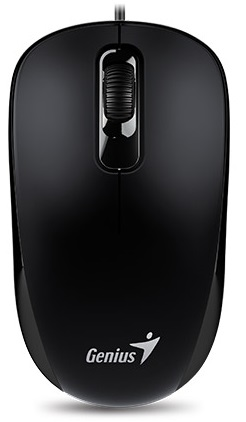
\includegraphics[width=.4\linewidth]{img/genius_mys.jpg}
  \caption{Fotka genius myši prevzatá z oficiálnej genius stránky~\cite{genius_mouse_pic}}
  \label{obr:uvod:genius:mouse:pic}
\end{subfigure}%
\begin{subfigure}{.5\textwidth}
  \centering
  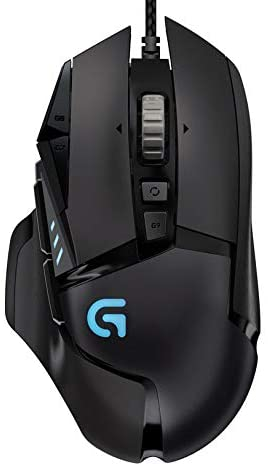
\includegraphics[width=.4\linewidth]{img/logitech_mys}
  \caption{Fotka logitech myši prevzatá zo stránky obchodu~\cite{logitech_mouse_pic}}
  \label{fig:sub2}
\end{subfigure}
\caption{Ukážka myší, ktorých input budeme porovnávať}
\label{obr:uvod:logitech:mouse:pic}
\end{figure}

Teraz si ukážeme ako sa líši ich input. Dáta budeme vyobrazovať pomocou obyčajného hexdumpu (zvýraznená časť v hexdumpe reprezentuje input zariadenia). Na oboch myšiach stlačíme ľavé tlačidlo a mierne ich posunieme smerom hore. Dáta, ktoré poslala genius myš sú vyobrazené na obrázku~\ref{obr:uvod:genius:input} a dáta poslané logitech myšou môžeme vidieť na obrázku~\ref{obr:uvod:logitech:input}.

\begin{figure}[!htb]
	\centering
	
\includegraphics[width=12cm]{img/uvod_genius_input}
	\caption{Ukážka hexdumpu so zvýrazneným inputom genius myši.}
	\label{obr:uvod:genius:input}
\end{figure}

\begin{figure}[!htb]
	\centering
	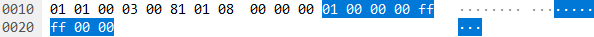
\includegraphics[width=12cm]{img/uvod_logitech_input}
	\caption{Ukážka hexdumpu so zvýrazneným inputom logitech myši.}
	\label{obr:uvod:logitech:input}
\end{figure}

Aj napriek tomu, že sa jedná o zariadenia z tej istej USB triedy a dokonca o rovnaké zariadenie -- myš,  má ich komunikácia rozličný tvar definovaný priamo výrobcom zariadenia. Analýzou \textit{Report Descriporu} (o ktorej si viac povieme neskôr v práci) sme zistili, že dáta, ktoré poslala genius myš majú nasledujúci význam:
\begin{itemize}
\item Byte 0: bity 0--2 reprezentujú stlačenie jednotlivých tlačidiel, bity 3--7 tvoria len dodatočnú výplň bytu
\item Byte 1: reprezentuje súradnicu X
\item Byte 2: reprezentuje súradnicu Y
\item Byte 3: reprezentuje koliesko myši
\end{itemize}

Pre porovnanie, význam dát poslaných logitech myšou je nasledovný:
\begin{itemize}
\item Byte 0--1: reprezentujú stlačenie jednotlivých tlačidiel
\item Byte 2--3: reprezentuje súradnicu X
\item Byte 4--5: reprezentuje súradnicu Y
\item Byte 6: reprezentuje koliesko myši
\item Byte 7: je rezervovaný výrobcom myši
\end{itemize}

Vizuálne zobrazený význam dát genius myši je ukázaný na obrázku~\ref{obr:uvod:genius:input:vyznam} a logitech myši na obrázku~\ref{obr:uvod:logitech:input:vyznam}.

\begin{figure}[!htb]
	\centering
	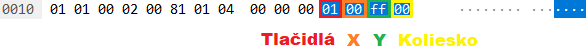
\includegraphics[width=12cm]{img/uvod_genius_input_vyznam}
	\caption{Ukážka hexdumpu so zvýrazneným inputom genius myši s významom.}
	\label{obr:uvod:genius:input:vyznam}
\end{figure}

\begin{figure}[!htb]
	\centering
	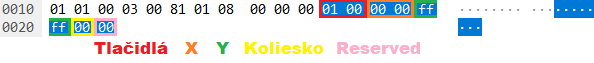
\includegraphics[width=12cm]{img/uvod_logitech_input_vyznam}
	\caption{Ukážka hexdumpu so zvýrazneným inputom logitech myši s významom.}
	\label{obr:uvod:logitech:input:vyznam}
\end{figure}

Z toho vyplýva, že aby sme boli schopní vykonať sémantickú analýzu HID zariadení, bude pre nás kľúčové vedieť rozparsovať \textit{Report Descripor} a na základe toho interpretovať input zariadení.

\section{Existujúce aplikácie}

Momentálne existuje niekoľko známych aplikácií ktoré slúžia na analýzu USB paketov. Ich predbežným skúmaním a používaním sme ale zistili, že úplne nevyhovujú našim konkrétnym požiadavkám. Avšak mnohé ich funkcie nám prídu užitočné a môžu poslúžiť ako inšpirácia v implementovaní našej aplikácie. V tejto kapitole si ukážeme výhody a nevýhody zopár aplikácií, ktoré sme si zvolili ako príklady v oblasti paket analyzátorov. Ich výber spočíval v tom, že sú veľmi rozšírené medzi verejnosťou a sú najbližšie k tomu čo by sme chceli od našej aplikácie.

Je nutné upozorniť, že väčšina dnešných analyzátorov sú platené aplikácie, prípadne majú odomknuté len základné vlastnosti s~možnosťou dokúpenia si plnej verzie. Práve preto sme nemali možnosť si pri všetkých vyskúšať ich celú funkcionalitu a na niektoré platené funkcie máme tak len ilustračný pohľad.


\subsection*{Wireshark}
\label{uvod:sec:Wireshark}

Aplikácia, ktorá na prvý pohľad nesúvisí s USB zbernicou. Wireshark je pravdepodobne najznámejší analyzátor a sniffer sieťových paketov. Jeho funkcionalita je veľmi rozsiahla, a~vzhľadom na~to, že sa jedná o~open-source projekt, neustále rastie. Vďaka jeho obecnému návrhu podporuje spoluprácu s~rôznymi inými sniffermi (LANalyzer, NetXRay a pod.). Jeden z~takýchto snifferov je \textit{USBPcap}, ktorý zachytáva USB komunikáciu a tým pádom je Wireshark schopný analyzovať pakety aj nad~touto zbernicou. 

Pre priblíženie niektorých funkcií Wiresharku si ukážeme analýzu komunikácie s USB myšou (Genius DX\=/120~\cite{genius_mouse}). Medzi tie úplne základné funkcie určite patrí hexdump dát nad~ktorými prebieha analýza, ktorý je vyobrazený na obrázku~\ref{obr:uvod:wireshark_hexdump}. 

\begin{figure}[!htb]
	\centering
	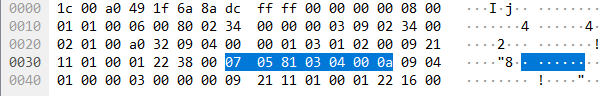
\includegraphics[width=12cm]{img/uvod_wireshark_hexdump}
	\caption{Ukážka hexdumpu vo Wiresharku.}
	\label{obr:uvod:wireshark_hexdump}
\end{figure}


Tento hexdump je tvorený dátami z jedného control prenosu, kde zariadenie posiela informácie o sebe samom v podobe rôznych descriptorov. 

V hexdumpe si takisto vieme pomocou kliknutia a ťahania myšou označiť ľubovoľné dáta, ktoré chceme. Zvýraznené byty na obrázku~\ref{obr:uvod:wireshark_hexdump_endpoint} reprezentujú jeden \textit{endpoint descriptor}.

\begin{figure}[!htb]
	\centering
	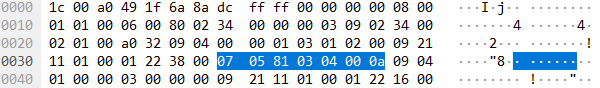
\includegraphics[width=12cm]{img/uvod_wireshark_hexdump_endpoint}
	\caption{Ukážka hexdumpu so zvýrazneným endpoint descriptorom.}
	\label{obr:uvod:wireshark_hexdump_endpoint}
\end{figure}

Pri pohybe myšou nad daným hexdumpom ponúka Wireshark interaktívnu odozvu, pričom farebne oddeľuje jednotlivé byty podľa ich významu. Na obrázku~\ref{obr:uvod:wireshark_hexdump_data_selection} vidíme konkrétny príklad -- ak podržíme myš nad hexa časťou bytu 00, automaticky nám to označí aj byte 04 pred ním, pretože spoločne reprezentujú jednotnú informáciu -- položku \textit{wMaxPacketSize} v \textit{endpoint descriptore}.

\begin{figure}[!htb]
	\centering
	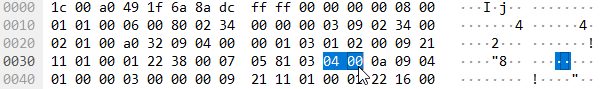
\includegraphics[width=12cm]{img/uvod_wireshark_data_selection}
	\caption{Ukážka hexdumpu s farebným oddelením na základe významu.}
	\label{obr:uvod:wireshark_hexdump_data_selection}
\end{figure}

Ďalšia užitočná vlastnosť je, že pri označení hexa znakov v hexdumpe, sa samé označia aj im odpovedajúce tlačiteľné znaky (obdobne to funguje aj opačným smerom). To, že vyššie označených 7 bytov na obrázku~\ref{obr:uvod:wireshark_hexdump_endpoint} reprezentujú \textit{endpoint descriptor} sme zistili vďaka špecifikácii jednotlivých descriptorov a vlastnou analýzou bytov v hexdumpe. Wireshark ale ponúka rozličné zobrazenie tých istých dát, a to napríklad aj pomocou stromovej štruktúry, ktorá už jednotlivým bytom pridáva ich sémantický význam v slovnom tvare ako je ukázané na obrázku~\ref{obr:uvod:tree_structure} nižšie.

\begin{figure}[!htb]
	\centering
	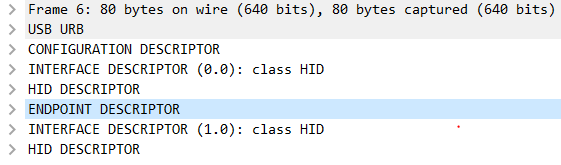
\includegraphics[width=11cm]{img/uvod_tree_structure}
	\caption{Ukážka reprezentácie dát pomocou stromovej štruktúry.}
	\label{obr:uvod:tree_structure}
\end{figure}

 Jednotlivé položky si môžeme bližšie rozbaliť. Napríklad vyššie zvýraznených 7 bytov reprezentujú konkrétny \textit{endpoint descriptor}, ktorý je ukázaný na obrázku~\ref{obr:uvod:endpoint}. Na tom istom obrázku si takisto môžeme všimnúť, že položka \textit{wMaxPacketSize} má hodnotu 4, čo je presne hodnota bytov 04 00, ktoré sme spomínali vyššie na obrázku~\ref{obr:uvod:wireshark_hexdump_data_selection}

\begin{figure}[!htb]
	\centering
	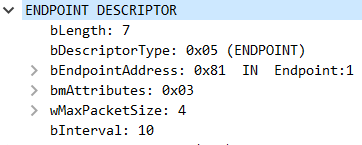
\includegraphics[width=8cm]{img/uvod_endpoint}
	\caption{Endpoint descriptor reprezentovaný dátami zvýraznenými na obrázku~\ref{obr:uvod:wireshark_hexdump} vyššie.}
	\label{obr:uvod:endpoint}
\end{figure}

Medzi viac špecifické funkcie patrí detailnejšie vyobrazenie jednotlivých bytov a~ich význam, ako je možné vidieť nižšie na~obrázku~\ref{obr:uvod:byte_detail_foto}. Na tomto obrázku vidíme rozbalenú položku \textit{bEndpointAddress}, ktorej hodnota je 0x81. Siedmy bit tejto hodnoty reprezentuje smer endpointu (IN -- slúži na prenos dát device $\longrightarrow$ host, OUT opačne) a dolné 4 bity označujú číslo endpointu. Túto vlastnosť aj napriek jej využitiu mnohé konkurenčné aplikácie postrádajú.

\begin{figure}[!htb]
	\centering
	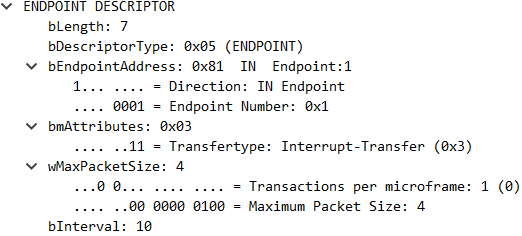
\includegraphics[width=8cm]{img/uvod_byte_detail}
	\caption{Ukážka vyobrazenia jednotlivých bytov.}
	\label{obr:uvod:byte_detail_foto}
\end{figure}

Wireshark ponúka interaktívne užívateľské rozhranie. V prípade kliknutia na konkrétny byte v hexdumpe sa nám označí jemu odpovedajúca položka v stromovej štruktúre. Príklad je ukázaný na obrázku~\ref{obr:uvod:hexdump_click}.

\begin{figure}[!htb]
	\centering
	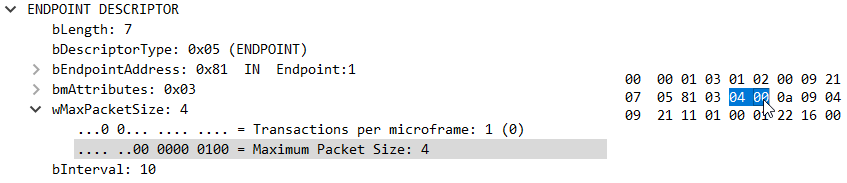
\includegraphics[width=\textwidth]{img/uvod_wireshark_hexdump_click}
	\caption{Ukážka kliknutia na položku v hexdumpe.}
	\label{obr:uvod:hexdump_click}
\end{figure}

Podobne to funguje aj opačne, takže ak klikneme na položku v stromovej štruktúre, označí sa jej odpovedajúca časť v hexdumpe. Príklad kliknutia na \textit{endpoint descriptor} v stromovej štruktúre a označenia jemu odpovedajúcej časti hexumpu je vidieť na obrázku~\ref{obr:uvod:tree_click}.

\begin{figure}[!htb]
	\centering
	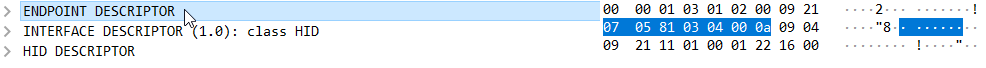
\includegraphics[width=\textwidth]{img/uvod_wireshark_tree_click}
	\caption{Ukážka kliknutia na položku \textit{endpoint descriptoru} v stromovej štruktúre.}
	\label{obr:uvod:tree_click}
\end{figure}

Obecné vyobrazenie pohybu paketov na zbernici bez hlbšej analýzy je ukázané na obrázku~\ref{obr:uvod:wireshark_listview} nižšie.

\begin{figure}[!htb]
	\centering
	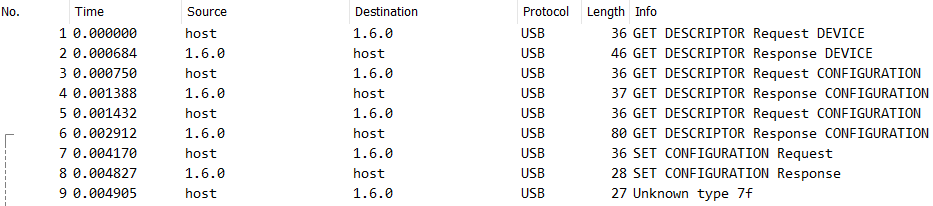
\includegraphics[width=\textwidth]{img/uvod_wireshark_listview}
	\caption{Príklad obecného vyobrazenia jednotlivých paketov vo Wiresharku.}
	\label{obr:uvod:wireshark_listview}
\end{figure}

Výhoda Wiresharku je hlavne v~tom, že podporuje širokú škálu descriptorov a~plná verzia programu je dostupná úplne zadarmo. Z~pohľadu užívateľa je až prekvapivé, že aj~napriek rozsiahlosti programu je aplikácia veľmi user-friendly orientovaná a~dopĺňa ju intuitívne užívateľské rozhranie.

Naopak, jeho nevýhodou je sčasti neprehľadný hexdump. Ako môžeme vidieť na obrázku~\ref{obr:uvod:wireshark_hexdump}, jedná sa o obyčajný hexdump, ktorý nijakým spôsobom neoddeľuje význam dát bez interakcie užívateľa. Preto v momente ak by sme nemali stromovú štruktúru k odpovedajúcemu hexdumpu, museli by sme sa riadiť špecifikáciou a vlastnou analýzou. V prípade rozsiahlejšieho hexdumpu môže byť veľmi obtiažné sa v ňom potom zorientovať. Ďalšia vec ktorá nám nevyhovuje, je chýbajúca sémantická analýza inputu rôznych zariadení. Ten je vyobrazený len pomocou hexdumpu a popisu \uv{Leftover Capture Data} ako je ukázané na obrázku~\ref{obr:uvod:wireshark_input}. Zo sekcie~\ref{uvod:sec:HID} nám je teda jasné, že vôbec netušíme čo jednotlivé dáta znamenajú, pretože ich význam je definovaný v \textit{Report Descriptore}.

\begin{figure}[!htb]
	\centering
	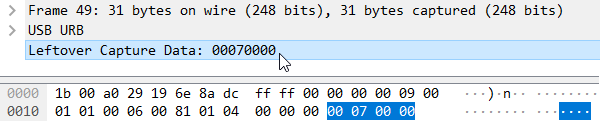
\includegraphics[width=12cm]{img/uvod_wireshark_input}
	\caption{Príklad inputu myši vo Wiresharku.}
	\label{obr:uvod:wireshark_input}
\end{figure}

\subsection*{Device Monitoring Studio}

Aplikácia ponúka analýzu sieťových a~USB paketov, tak ako aj~analýzu komunikácie prebiehajúcej cez~sériový port. Zároveň slúži aj ako sniffer na všetkých týchto portoch.

Ako prvé na~aplikácii zaujme spôsob zvolenia si zariadenia s~ktorým bude sledovaná komunikácia. Je implementovaný štýlom stromovej štruktúry ako je ukázané na~obrázku~\ref{obr:uvod:hhd_treeview_foto}~nižšie, kde máme konkrétne označenú rovnakú myš s ktorou komunikáciu sme sledovali predchádzajúcim programom. 

\begin{figure}[!htb]
	\centering
	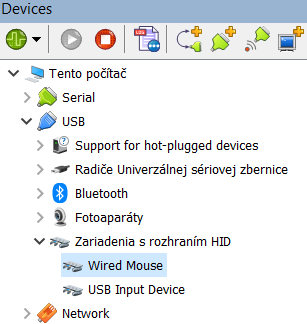
\includegraphics{img/uvod_hhd_treeview}
	\caption{Ukážka stromovej štruktúry na~zvolenie si zariadenia, s~ktorým bude zachytávaná komunikácia.}
	\label{obr:uvod:hhd_treeview_foto}
\end{figure}

Základná verzia programu ponúka vizuálne zobrazenie \textit{URB}, tak ako aj analýzu jednotlivých paketov.
Pod analýzou si tu môžeme predstaviť ale len obyčajný hexdump, ktorý neposkytuje žiadne významové oddelenie dát a tým pádom je obtiažnejšie sa v ňom zorientovať. Príklad môžeme vidieť na obrázku~\ref{obr:uvod:hhd_hexdump}.

\begin{figure}[!htb]
	\centering
	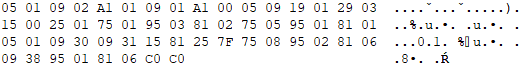
\includegraphics[width=12cm]{img/uvod_hhd_hexdump}
	\caption{Príklad hexdumpu v Device Monitoring Studio.}
	\label{obr:uvod:hhd_hexdump}
\end{figure}


Takisto tu nemáme kompletné sémantické vysvetlenie čo dané dáta znamenajú (napríklad pomocou stromovej štruktúry ako to rieši konkurencia). K dispozícii máme len veľmi obmedzený popis jednotlivých paketov (číslo paketu, device request, a pod.), pričom ani nie je veľmi jasné odkiaľ sa tieto informácie vzali. Príklad takéhoto popisu aj s hexdumpom je ukázaný na obrázku~\ref{obr:uvod:hhd_analyza}~nižšie.

\begin{figure}[!htb]
	\centering
	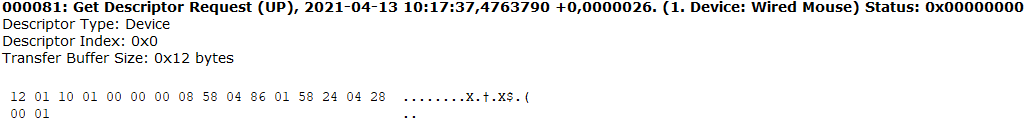
\includegraphics[width=\textwidth]{img/uvod_hhd_analyza}
	\caption{Príklad analýzy paketov.}
	\label{obr:uvod:hhd_analyza}
\end{figure}


Vyobrazenie \textit{URB} (obrázok~\ref{obr:uvod:hhd_urb}~) tak ponúka súhrn týchto popisov jednotlivých paketov, ktoré sú postupne zachytené počas komunikácie na zbernici.

\begin{figure}[!htb]
	\centering
	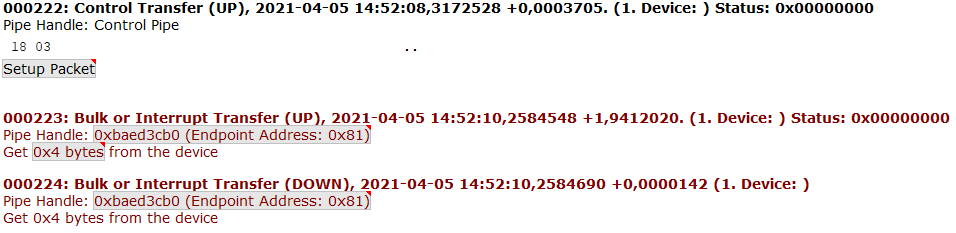
\includegraphics[width=\textwidth]{img/uvod_hhd_urb}
	\caption{Ukážka vyobrazenia URB.}
	\label{obr:uvod:hhd_urb}
\end{figure}

Pričom pri dvojkliku na šedé časti textu (napríklad \textit{Setup Packet} alebo \textit{Endpoint Address}) sa užívateľovi rozbalí okno s detailnejším popisom.
 
Analýza inputu myši, ktorú môžeme vidieť na obrázku~\ref{obr:uvod:hhd_input}, je riešená podobným spôsobom ako pri analýze descriptorov.

\begin{figure}[!htb]
	\centering
	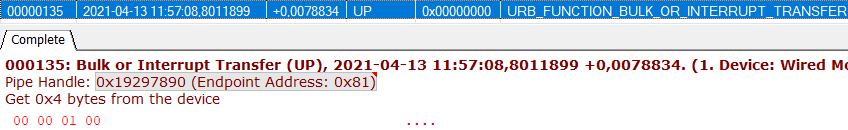
\includegraphics[width=\textwidth]{img/uvod_hhd_input}
	\caption{Príklad inputu myši v Device Monitoring Studio.}
	\label{obr:uvod:hhd_input}
\end{figure}

Obecné vyobrazenie jednotlivých paketov bez bližšej analýzy je riešené podobne ako vo Wiresharku, pričom pakety sú farebne oddelené podľa ich smeru pohybu na zbernici (posielané smerom host $\longrightarrow$ zariadenie/smerom zariadenie $\longrightarrow$ host). Toto je veľmi pekná funkcionalita, ktorá celkovo sprehľadňuje komunikáciu zariadenia s hostom. Príklad je ukázaný na obrázku~\ref{obr:uvod:hhd_listview}.

\begin{figure}[!htb]
	\centering
	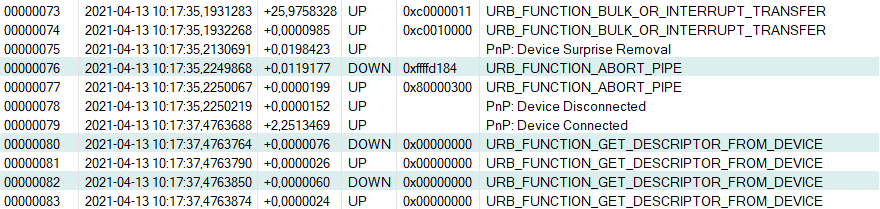
\includegraphics[width=\textwidth]{img/uvod_hhd_listview}
	\caption{Príklad obecného vyobrazenia jednotlivých paketov v Device Monitoring Studio.}
	\label{obr:uvod:hhd_listview}
\end{figure}

Zaujímavá funkcionalita, ktorú ale program ponúka len v platenej verzii, je umožnenie užívateľovi priamo komunikovať so zvoleným zariadením. Môžeme mu tak posielať rôzne požiadavky (niektoré z nich sú spomenuté v USB 2.0 špecfikácii\cite{usbdoc} v kapitole 9.4) ako napríklad \textit{GET\_REPORT} kde špecifikujeme \textit{Report ID} a prípadné ďalšie parametre, a zariadenie nám patrične odpovie.

Užívateľské rozhranie vyobrazené nižšie pomocou obrázku~\ref{obr:uvod:hhd_interface}~,pozostáva z pomerne veľa ikoniek a celkovo sa javí ako trochu neprehľadné. Pri prvotnej interakcii s programom chvíľu trvá, kým človek nájde čo~i~len základné informácie ako napríklad hlavičky ku~jednotlivým paketom. Nepoteší ani fakt, že verzia zadarmo nedovoľuje monitorovanie dlhšie ako 10 minút a~maximálny počet monitorovaní za~jeden deň je taktiež 10.

\begin{figure}[!htb]
	\centering
	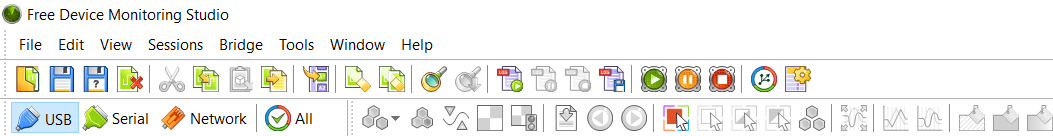
\includegraphics[width=\textwidth]{img/uvod_hhd_interface}
	\caption{Užívateľské rozhranie Device Monitoring Studio.}
	\label{obr:uvod:hhd_interface}
\end{figure}


\section{Požadované funkcie}

Ako prvé by sme si mali zadefinovať platformu na ktorú budeme cieliť s našou aplikáciou:
\begin{enumerate}[label=\textbf{P\arabic*}]
	\item \label{uvod:poz:platforma} Cieľová platforma našej aplikácie by mala byť Windows. 
\end{enumerate}

Keďže má naša aplikácia mať výukový charakter, tak sa pozrieme na typický výukový scénár jej používania. Učiteľ si dopredu do súboru zachytí komunikáciu s určitým zariadením na ktorej overí, že je didakticky dobrá a ilustruje to čo má. Následne daný súbor posunie študentom aby si mohli zobraziť analýzu konkrétnych paketov. Užitočná je ale aj analýza priamej interakcie užívateľa s jeho konkrétnym zariadením, preto by sme zároveň chceli podporovať aby si študenti mohli pripojiť vlastné zariadenie a skúmať s ním komunikáciu v reálnom čase. Z toho nám vyplývajú naledujúce požiadavky:
\begin{enumerate}[label=\textbf{P\arabic*},resume]
	\item \label{uvod:poz:analyza} Mala by byť schopná analyzovať USB pakety zachytené do~súboru v~rozumnom formáte pomocou predom definovaného snifferu.
	\item \label{uvod:poz:analyza_real_time} Mala by byť schopná analýzy paketov v reálnom čase. To znamená, že bude podporovať čítanie súboru súvisle s tým ako do neho bude zapisovať iný software (za predpokladu, že to daný software povoľuje).
\end{enumerate}

Ako sme mohli vidieť aj na predchádzajúcich príkladoch, hexdump je jednou zo základných funkcií na analýzu paketov. Zároveň sa nám ale nepáčilo, že väčšina hexdumpov je neprehľadná a ťažko sa v nich orientuje. Preto si zadefinujeme nasledujúce požiadavky:
\begin{enumerate}[label=\textbf{P\arabic*},resume]
	\item \label{uvod:poz:hexdump} Mala by pomocou hexdumpu vedieť zobraziť dáta, ktoré daný sniffer zachytí a~uloží.
	\item \label{uvod:poz:data_highlight} Mala by mať prehľadnejší hexdump a užívateľovi uľahčiť orientáciu v~ňom. Jednotlivé znaky by mali byť farebne označené na~základe ich významu (hlavička paketu, rôzne typy descriptorov a pod.).
\end{enumerate}

K sémantickej analýze sa nám môže hodiť vedieť zobraziť dáta a ich význam pomocou stromovej štruktúry. Pretože sa s našou aplikáciou budeme snažiť vysvetliť základy komunikácie na USB zbernici, mali by sme podporovať sémantickú analýzu všetkých základných USB descriptorov a takisto inputu určitej podmnožiny HID zariadení. Ako posledné by sa nám zišlo vedieť pomocou stromovej štruktúry vyobraziť hlavičku jednotlivých paketov. Z toho celého dostávame nasledovné:
\begin{enumerate}[label=\textbf{P\arabic*},resume]
	\item \label{uvod:poz:descriptory} Mala by podporovať sémantickú analýzu (vyobrazenie pomocou stromovej štruktúry) pre~všetky základné USB descriptory spomenuté v~USB 2.0 špecifikácii\cite{usbdoc} v kapitole 9.6~(ako napríklad \textit{Device descriptor}, \textit{Interface descriptor}, \textit{Endpoint descriptor}, atď.).
	\item \label{uvod:poz:hid_analyza} Mala by byť schopná pomocou stromovej štruktúry zobraziť sémantický význam dát posielaných danou podmnožinou HID zariadení, do~ktorej patrí myš, klávesnica a~joystick.
	\item \label{uvod:poz:paket_hlavicka} Mala by byť schopná pomocou stromovej štruktúry zobraziť sémantický význam jednotlivých hlavičiek paketov.
\end{enumerate}

Vyššie v texte sme označili funkciu Wiresharku vyobraziť sémantický význam dát na bitovej úrovni (obrázok~\ref{obr:uvod:byte_detail_foto}) za zaujímavú. Preto by sme ju chceli implementovať aj v našej aplikácii, z čoho vyplýva:
\begin{enumerate}[label=\textbf{P\arabic*},resume]
\item \label{uvod:poz:show_bits} V~miestach kde to dáva zmysel, by aplikácia mala byť schopná zobrazovať význam dát až na~úrovni jednotlivých bitov.
\end{enumerate}

Nechceme užívateľov hneď zaplaviť všetkými detailnými informáciami o paketoch. Preto by sme mali vedieť zobraziť zopár obecných vecí ku každému paketu a vyobraziť tak pohyb na zbernici, a až v prípade interakcie užívateľa s aplikáciou zobraziť podrobný popis jednotlivých paketov. Zároveň sa nám páčila funkcia Device Monitoring Studia, kde boli jednotlivé pakety farebne rozlišiteľné, čo zvyšovalo celkový prehľad pohybu paketov na zbernici. Z toho dostávame nasledujúce požiadavky:
\begin{enumerate}[label=\textbf{P\arabic*},resume]
	\item \label{uvod:poz:zobrazenie_paketov} Mala by na prvý pohľad jasne zobraziť základné informácie o~každom analyzovanom pakete (ako napr. dĺžka paketu, typ prenosu a pod.) a~pri~bližšom skúmaní jednotlivých paketov detailnejšie zobraziť celú jeho hlavičku. Tieto základné informácie by mali byť farebne rozlišiteľné na základe smeru paketu po zbernici.
	\item \label{uvod:poz:paket_detail} Detailnejšie informácie o~pakete budú zobrazované na~základe interakcie užívateľa s~aplikáciou.
\end{enumerate}

Aby sme boli schopní sémantickej analýzy dát myši, klávesnice alebo joysticku podľa osobného výberu užívateľa, musíme si získať informácie o ich inpute z \textit{HID Report Descriptoru}, takže naša ďalšia požiadavka je:
\begin{enumerate}[label=\textbf{P\arabic*},resume]
	\item \label{uvod:poz:report_desk_parser} Mala by byť schopná rozparsovať \textit{HID Report Descriptor} takým štýlom, aby bolo neskôr možné sématnicky reprezentovať input nami zvolených HID zariadení -- myš, klávesnica a joystick.
\end{enumerate}

\section{Ciele práce}

Celkové ciele tejto práce sú následovné :

\begin{enumerate}[label=\textbf{C\arabic*}]
	\item \label{uvod:ciel:aplikacia} Naprogramovať funkčný analyzátor, ktorý spĺňa všetky požadované funkcie~\ref{uvod:poz:platforma}\=/\ref{uvod:poz:report_desk_parser}
	\item \label{uvod:ciel:rozsiritelnost} Návrh programu musí byť dostatočne obecný aby splňoval nasledujúce:
	\begin{itemize}
		\item \label{uvod:ciel:roz_USB} Jednoduché rozšírenie o~analýzu ďalších typov USB prenosov.
		\item \label{uvod:ciel:roz_HID} Jednoduché pridanie sémantickej analýzy pre~ďalšie HID zariadenia.
	\end{itemize}
\end{enumerate}
\chapter{USB}
V tejto kapitole si rozšírime znalosti fungovania USB, ktoré sme získali v sekcii~\ref{uvod:sec:zakl_pojmy}. Najprv si vysvetlíme ako prebieha komunikácia medzi USB zariadením a hostom, následne sa pozrieme na konfiguráciu USB zariadenia po pripojení na zbernicu, prejdeme si niektoré základné USB descriptory a ako posledné si ešte vysvetlíme základnú stavbu USB na Windowse.

\section{Komunikácia}
Detailný popis komunikácie a presunu dát po zbernici je opísaný v USB 2.0 špecifikácii v kapitole 5~\cite{usb_chap5}. My sa momentálne zameriame len na určité časti, ktoré sú potrebné pre našu prácu. Každé USB zariadenie v sebe obsahuje tzv. \textit{endpointy}~\cite{usb_chap5_endpoint} -- môžeme to považovať za akúsi koncovku komunikácie medzi hostom a zariadením. Koncepčne sa jedná o schopnosť zariadenia v sebe uchovať dáta (memory buffer). Ako už vieme z kapitoly~\ref{uvod:sec:zakl_pojmy}, komunikáciu riadi USB host, a tá prebieha práve pomocou týchto endpointov -- v prípade ak chce host poslať určité dáta zariadeniu, zapíše ich do jeho konkrétneho endpointu. V prípade ak chce zariadenie poslať určité dáta hostovi, zapíše si ich do daného endpointu, odkiaľ ich host potom prečíta.

\subsection*{Endpoint}
\label{kap02:sec:endpoint}
USB zariadenie typicky pozostáva z niekoľkých na sebe nezávislých endpointov. Každý endpoint je potom jednoznačne určený:
\begin{enumerate}
\item Adresou USB zariadenia -- tá je pridelená USB zariadeniu pri jeho konfigurácii v momente pripojenia na zbernicu.
\item Číslom endpointu -- unikátne číslo, ktoré určuje výrobca zariadenia.
\item Smerom prenosu dát -- host $\longrightarrow$ device alebo device $\longrightarrow$ host.
\end{enumerate}

Do momentu pokiaľ neprebehne konfigurácia USB zariadenia a jeho endpointov, sú endpointy s adresou inou ako 0 v neurčitom stave a nemusia byť pre hosta dostupné. Endpoint s adresou 0, inak nazývaný aj ako \uv{default endpoint} alebo \uv{Endpoint0}, slúži na nakonfiguranie daného USB zariadenia. Výrobca zariadenia je povinný poskytnúť aspoň 1 Endpoint0 pre každý smer pohybu dát, prípadne 1 Endpoint0 s možnosťou prenosu oboma smermi. Funkcie (USB zariadenia) môžu obsahovať aj ďalšie endpointy s adresou inou ako 0. Tieto endpointy slúžia na prenos dát špecifických pre dané zariadenie (napríklad na posielane inputu myši). Rôzne endpointy môžeme zlučovať do určitých množín podľa ich funkcionality. Takúto množinu endpointov potom nazývame \textit{interface}. Niektoré USB zariadenia potom môžu pozostávať z viacerých interfacov, ktoré budú reprezentovať rozličné USB triedy.

\subsection*{Pipe}
USB pipe~\cite{usb_chap5_pipe} je termín označujúci spojenie medzi konkrétnym endpointom USB zariadenia a Host Controllerom (interface medzi hostom a zbernicou). Reprezentuje schopnosť prenášať dáta medzi hostom a endpointom pomocou memory bufferu. Pipe ktorá pozostáva z dvoch Endpoint0 sa nazýva \uv{Default Control Pipe} a je prístupná v momente pripojenia zariadenia na zbernicu a slúži na konfiguráciu daného zariadenia (po konfigurácii môže mať aj iné využitie, ktoré špecifikuje samotný výrobca). Ostatné pipy s ďalšími endpointami (za predpokladu, že existujú) sú vytvorené až po konfigurácii zariadenia. 



\section{Konfigurácia}
Konfigurácia USB zariadenia je detailne opísaná v USB 2.0 špecifikácii~\cite{usb_chap9_conf}. Predtým ako začneme využívať funkcionalitu pripojeného USB zariadenia, je USB host zodpovedný za jeho nakonfigurovanie. Počas konfigurácie posiela USB host zariadeniu tzv. \uv{Device Requesty}, na ktoré dané zariadenie odpovedá cez Default Control Pipe. Tieto requesty sú špecifikované v \textit{Setup Pakete} -- štruktúra veľká 8 bytov so štandardným formátom definovaným v USB špecifikácii 2.0~\cite{usb_chap9_setup_pak}. Existuje niekoľko základných requestov~\cite{usb_chap9_device_req}, na ktoré musí každe USB zariadenie vedieť reagovať. Patria medzi ne napríklad:
\begin{itemize}
\item Get Descriptor -- vypýta si od zariadenia konkrétny descriptor, ktorý mu zariadenie pošle ako odpoveď na tento request (za predpokaldu, že daný descriptor existuje)
\item Set Configuration -- nastaví konkrétnu konfiguráciu zariadeniu
\end{itemize}

Bežný postup konfigurácie je, že si USB host vypýta rôzne descriptory od zariadenia, ktoré určujú jeho schopnosti (napr. \textit{Configuration Descriptor}, \textit{Interface Descriptor}, \textit{Endpoint Desriptor}) a potom pomocou requestu Set Configuration nastaví požadovanú konfiguráciu (a ak je to nutné, zvolí rôzne dodatočné nastavenie interfacov).



\section{USB Descriptory}
Teraz si prejdeme niekoľko základných USB descriptorov a ich jednotlivé položky, pretože ich význam budeme potrebovať neskôr v tejto práci. 


\subsection*{Configuration Descriptor}
Configuration Descriptor~\cite{usb_chap9_conf_desc} opisuje informácie o konkrétnej konfigurácii USB zariadenia. Obsahuje položku \textit{bConfigurationValue} -- číslo reprezentujúce konkrétnu konfiguráciu, ktorú USB host použije ako parameter\newline v~\texttt{SetConfiguration()} requeste v prípade, že chce nastaviť práve túto konfiguráciu. Každé zariadenie má aspoň jeden Configuration Descriptor. Každá konfigurácia obsahuje aspoň jeden interface a každý interface má nula alebo viac endpointov. V prípade, že si host vyžiada od zariadenia Configuration Descriptor, dostane spolu s ním aj všetky súvisiace Interface a Endpoint descriptory.


\subsection*{Interface Descriptor}
Interface Descriptor~\cite{usb_chap9_interf_desc} opisuje šepcifický interface konkrétnej konfigurácie USB zariadenia. Ak zariadenie podporuje viac ako jeden interface, tak všetky Interface Descriptory spolu s im odpovedajúcimi Endpoint Descriptormi sú vrátené ako odpoveď na \texttt{GetConfiguration()} request (k Interface Descriptoru nie je možný priamy prístup pomocou \texttt{GetDescriptor()} alebo \texttt{SetDescriptor()} requestom). Ak interface používa len Endpoint0, tak za Interface Descriptorom nenasleduje žiaden Endpoint Descriptor. Endpoint0 takisto nie je započítaný v položke Interface Descriptoru \textit{bNumEndpoints}, ktorá udáva počet endpointov konkrétneho interfacu.


\subsection*{Endpoint Descriptor}
Endpoint Descriptor~\cite{usb_chap9_end_desc} poskytuje hostovi informácie o konkrétnom endpointe. Tento descriptor obsahuje aj informácie na základe ktorých je host schopný určiť bandwidth konkrétneho endpointu -- množstvo dát prenesených za jednotku času (typicky bity za sekundu = b/s, alebo byty za sekundu = B/s). Takisto ako aj  pri Interface Descriptore, nie je možné k nemu priamo pristupovať pomocou \texttt{GetDescriptor()} alebo \texttt{SetDescriptor()} requestov, ale je súčasťou odpovede na \texttt{GetConfiguration()} request.

\section{Windows}
Keďže Windows je hlavná platforma na ktorú mierime s našou aplikáciou, priblížime si ako sú reprezentované jednotlivé USB zariadenia a priebeh komunikácie na danej zbernici.

Nasledujúca sekcia poskytuje zjednodušený popis a čerpá (pokiaľ nie je uvedené inak) z toho čo sa nachádza v Microsoft dokumentácii~\cite{usb_msdn_device_node_stack}.
Windows organizuje zariadenia pomocou stromovej štruktúry nazývanej \uv{Plug and Play device tree} alebo jednoducho len \uv{device tree}. Správca stromu sa nazýva \uv{PnP manager}~\cite{usb_msdn_pnp_manager}. Vrchol v tomto strome (tzv. \uv{device node}) reprezentuje USB zariadenie alebo nejakú jeho konkrétnu Funkciu. Koreň stromu obecne nazývame \uv{root device node} a typicky sa v diagramoch kreslí na spodku. Príklad takéhoto diagramu môžeme vidieť na obrázku~\ref{obr:kap2:device_tree} nižšie.

\begin{figure}[!htb]
	\centering
	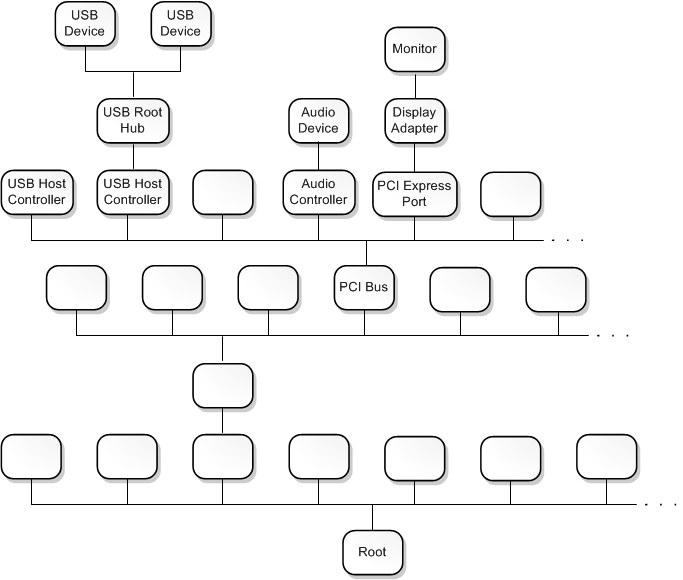
\includegraphics[width=10cm]{img/kap02_device_tree}
	\caption{Ukážka device tree. Obrázok prevzatý z Microsoft dokumentácie~\cite{usb_msdn_device_node_stack}}
	\label{obr:kap2:device_tree}
\end{figure}

Niektoré vrcholy môžu reprezentovať zbernice samotné, pričom synovia daného vrcholu zase reprezentujú zariadenia pripojené na túto zbernicu.

Windows má definovanú \texttt{DEVICE\_OBJECT} štruktúru~\cite{usb_msdn_device_object} reprezentujúcu \textit{device object} -- logické, virtuálne alebo fyzické zariadenie, ktoré využíva driver na spracovávanie I/O (input/output) requestov. Každý device node obsahuje usporiadaný list takýchto device objectov.  Usporiadaný list device objectov spolu s ich asociovanými drivermi nazývame \textit{device stack} (môžeme si to predstaviť ako stack dvojíc \textit{device object}$\leftrightarrow$driver). Tento stack má podľa konvencie vrch aj spodok -- prvé zariadenie ktoré bolo vytvorené na stacku sa nachádza na spodku a posledné vytvorené je naopak na vrchu. Ukážeme si to na konkrétnom príklade, kde na nasledujúcom obrázku~\ref{obr:kap2:device_node_diagram} môžeme vidieť device node s názvom \uv{Proseware Gizmo}, ktorého device stack obsahuje 3 položky: Vrchný device object má asociovaný \uv{AfterThought.sys} driver, stredný device object je spojený s driverom \uv{Proseware.sys} a posledný má zase \uv{Pci.sys} driver. Device stack \uv{PCI Bus} device nodu obsahuje len 2 položky: device node s \uv{Pci.sys} driverom a device node s \uv{Acpi.sys} driverom.

\begin{figure}[!htb]
	\centering
	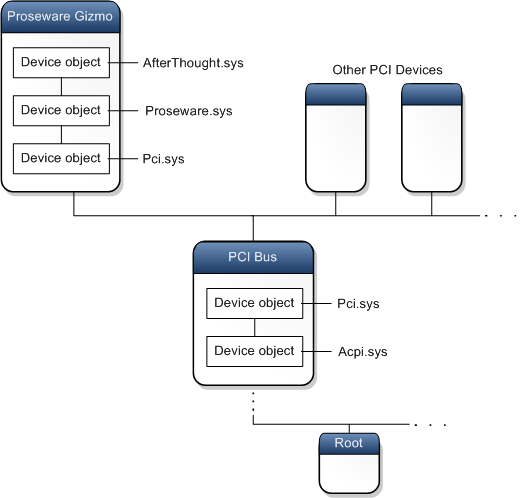
\includegraphics[width=10cm]{img/kap02_device_node_diagram}
	\caption{Ukážka konkrétnych device nodov. Obrázok prevzatý z Microsoft dokumentácie~\cite{usb_msdn_device_node_stack}}
	\label{obr:kap2:device_node_diagram}
\end{figure}

Konštrukcia tohto stacku je nasledovná:
\begin{itemize}
\item PnP manager poverí driver každej zbernice (v našom konkrétnom príklade z obrázku~\ref{obr:kap2:device_node_diagram} by to bol Pci.sys driver) aby sčítala všetky zariadenia, ktoré sú na ňu pripojené.
\item Ako odpoveď na túto požiadavku vytvorí driver danej zbernice device object pre každé pripojené zariadenie, ktorý nazývame \uv{physical device object (PDO)}. V príklade s Pci.sys driverom by to vyzeralo nasledovne:

\begin{figure}[!htb]
	\centering
	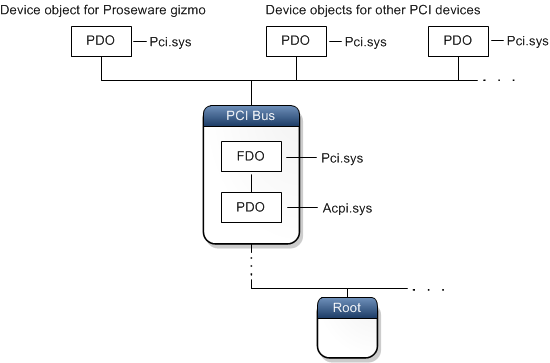
\includegraphics[width=10cm]{img/kap02_PDO}
	\caption{Ukážka vytvorenia konkrétnych PDO Pci.sys driverom. Obrázok prevzatý z Microsoft dokumentácie~\cite{usb_msdn_device_node_stack}}
	\label{obr:kap2:pdo}
\end{figure}

\item PnP manager pripradí device node každému novo vytvorenému PDO a pozrie sa do registru, aby zistil aké drivery majú byť súčasťou device stacku daného nodu. Každý device stack musí obsahovať práve jeden \textit{function driver} (hlavný driver device stacku, je zodpovedný za riadenie read, write a control requestov) a nula alebo viac \textit{filter driverov} (Ponúkajú prídavné možnosti v spracovávaní read, write a control requestov. Napríklad môžu meniť dáta, ktoré sú posielané daným requestom).
\item Akonáhle sú všetky drivery načítané, každý z nich vytvorí odpovedajúci device object a pripojí ho na daný device stack. Device object vytvorený function driverom nazývame \uv{functional device object (FDO)} a device objet vytvorený filter driverom zase \uv{filter device object (Filter DO)}. Náš konkrétny device tree vyobrazený na obrázku~\ref{obr:kap2:concrete_dev_tree} by teda vyzeral ako na obrázku~\ref{obr:kap2:concrete_dev_tree}.

\begin{figure}[!htb]
	\centering
	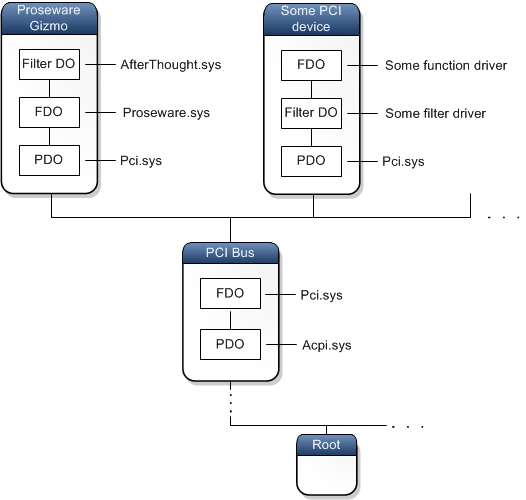
\includegraphics[width=10cm]{img/kap02_concrete_dev_tree}
	\caption{Ukážka konkrétneho device tree pre PCI zbernicu. Obrázok prevzatý z Microsoft dokumentácie~\cite{usb_msdn_device_node_stack}}
	\label{obr:kap2:concrete_dev_tree}
\end{figure}

\end{itemize}


Ako is ešte môžeme všimnúť na obrázku~\ref{obr:kap2:concrete_dev_tree}, v device node Proseware Gizmo je fitler driver (AfterThought.sys) nad function driverom (Proseware.sys). V takomto prípade je daný filter driver nazývaný \uv{upper filter driver}. Naopak v druhom device node (Some PCI device) je filter driver pod function driverom -- takýto filter driver nazývame \uv{lower filter driver}.

Keďže sú pre našu aplikáciu dôležité hlavne HID zariadenia, pozrieme sa teraz na to ako vyzerá driver stack a celková architektúra pre túto triedu zariadení~\label{kap02:sec:hid_arch}. Základom každého device stacku HID zariadenia je class driver \textit{hidclass.sys}, za ktorým nasledujú už konkrétne function/filter drivery. Príklad device stacku myši a klávesnice, tak ako aj HID triedy môžeme vidieť na nasledujúcom obrázku~\ref{obr:kap2:concrete_dev_stack}:

\begin{figure}[!htb]
	\centering
	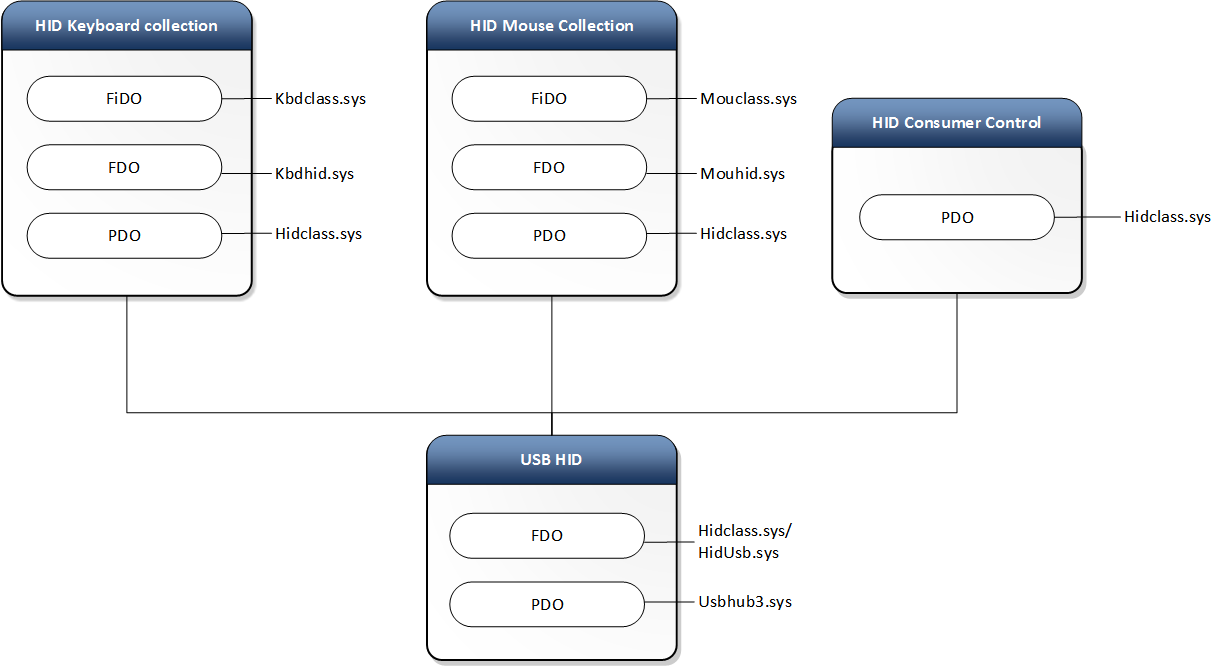
\includegraphics[width=\textwidth]{img/kap02_concrete_device_stack}
	\caption{Ukážka konkrétneho device stacku myši a klávesnice. Obrázok prevzatý z Microsoft dokumentácie~\cite{usb_msdn_hid_architecture}}
	\label{obr:kap2:concrete_dev_stack}
\end{figure}

Momentálne si vysvetlíme ešte zopár pojmov, ktoré sa nám budú hodiť neskôr v texte. \uv{HID Client}~\cite{usb_msdn_hid_client} je termín ktorým označujeme driver, service~\cite{usb_msdn_service} alebo aplikáciu, ktorá komunikuje s \textit{hidclass.sys} a často reprezentuje konkrétne zariadenie (napríklad myš alebo klávesnicu). \uv{Preparsed Data}~\cite{usb_msdn_preparsed_data} reprezentujú dáta Report Descriptoru asociované s konkrétnym zariadením. Aplikácie ich využívajú aby z nich vytiahli informácie o danom zariadení bez nutnosti parsovania Report Descriptoru.
\chapter{Analýza}
\section{Získanie USB packetov}
Na získavanie USB paketov nám bude obecne slúžiť paket sniffer. Väčšina paket analyzátorov má implementované vlastné sniffery a preto sme sa o to pokúsili tiež. Narazili sme ale na niekoľko zásadných problémov, ktoré sa úzko viažu s platformou na ktorú cielime s našou aplikáciou~--~Windows.

Microsoft dokumentácia podrobnejšie opisuje komunikáciu medzi HID zaridením a kernel/user-mode aplikáciou~\cite{hid_opening_collections}. Keďže naša aplikácia beží v user-mode, prejdeme si tento spôsob:
\begin{enumerate}
\item Aplikácia nájde a identifikuje HID zariadenie.
\item Aplikácia pomocou metódy \textit{CreateFile} otvorí spojenie s HID zariadením.
\item Aplikácia pomocou \textit{HID API}~\cite{hid_api} metód \textit{HidD\_Xxx} získa \textit{Preparsed Data} a informácie ohľadom HID zariadenia.
\item \textbf{Aplikácia použije metódu \textit{ReadFile} resp. \textit{WriteFile} na získanie inputu zariadenia resp. poslanie reportu zariadeniu.}
\item Aplikácia pomocou \textit{HID API}~\cite{hid_api} metód \textit{HidP\_Xxx} interpretuje HID reporty.
\end{enumerate}

\subsection{Windows exclusive mód}
Windows má definovaný tzv. \textit{Access Mode}, ktorý určuje restrikciu prístupu \textit{HID Clienta} k HID zariadeniu. 
Ten môže byť buď \textit{Shared} alebo \textit{Exclusive}. \textit{Exclusive Mode} zabraňuje ostatným \textit{HID Clientom} v zachytávaní alebo získavaní inputu HID zariadenia, pokiaľ nie sú hlavným príjemcom daného inputu. Preto z bezpečnostných dôvodov otvára \textit{RIM (Raw Input Manager)} niektoré zariadenia v \textit{Exclusive Mode}.

Ak je zariadenie otvorené v \textit{Exclusive Mode}, aplikácia má stále prístup k niektorým jeho údajom pomocou  \textit{HID API}~\cite{hid_api} metód  \textit{HidD\_\textbf{Get}Xxx}. Tieto metódy nám obecne umožnia získať niektoré descriptory zariadenia, tak ako aj jeho \textit{Preparsed Data}. Nie je nám ale umožnené volať metódu \textit{ReadFile}, takže nemáme akým spôsobom zachytávať komunikáciu HID zariadenia s clientom.

Tabuľka zariadení~\cite{hid_access} (obrázok~\ref{obr:kap3:access_mode}), ktoré \textit{RIM} otvára v \textit{Exclusive Mode} obsahuje aj tie, ktoré sme si v úvode zvolili ako podmnožinu HID zariadení na analýzu -- myš a klávesnica.

\begin{figure}[!htb]
	\centering
	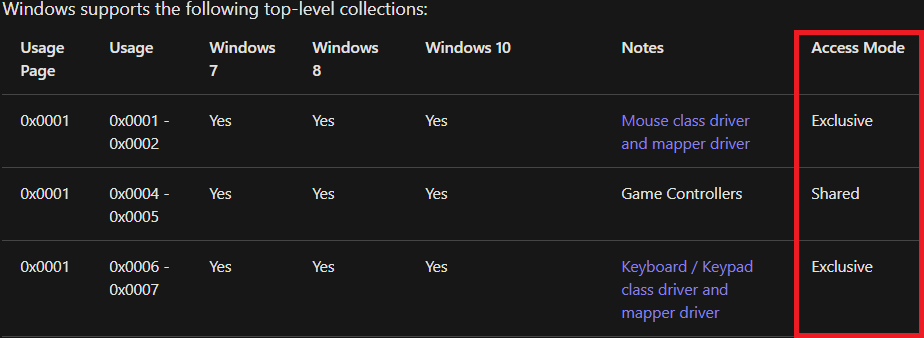
\includegraphics[width=\textwidth]{img/kap3_access_mode}
	\caption{Tabuľka zariadenía ich \textit{Access Mode}. Zariadenia postupne po riadkoch -- myš, joystick a klávesnica}
	\label{obr:kap3:access_mode}
\end{figure}

\newpage

\subsection{Známe knižnice}
opisat zakladne kniznice na sledovanie USB zbernice a preco som ich nemohol pouzit : libUSB, hidAPI

\subsection{Driver}
TU povedat riesenie - pouzitie driveru na komunikaciu so zariadenim. Existujuce windows drivery -- moufiltr, Kbdfiltr - nefunguju pre USB

TU spomenut posledne mozne riesenie - napisanie vlastneho filter driveru. 

\subsection{Third-party aplikácie}
opisat odkial nakoniec ziskavam packety - USBPcap a Wireshark









\section{Spracovávanie pcap súborov}
moznosti ako citat pcap subory : bud pouzit uz existujucu kniznicu : na linuxe Libpcap, windows NPcap(deprecated WinPcap), alebo citat subory manualne : std::istream alebo QFile
\section{Sémantická reprezentácia dát}
ako si z dat vytiahnut udaje ktore su potom pouzite na semanticku analyzu implementovanych HID zariadeni : HID Report parser, InputValues a EndpointDevice struct.
Nasledne sparovanie - ako vybrat spravny report pre konkretny input
\section{Voľba frameworku}
obecne co by som od toho GUI priblizne chcel, potom opisat preco som si vybral prave Qt a v nasledujucich kapitolach opisat rozhodnutia uz v Qt
dovod preco som si zvolil qt namiesto inych c++ GUI frameworkov(napriklad sfml)
\section{Zobrazenie základných informácií}
ako zobrazovat zakladne info o packete : pouzit QListWidget alebo QTableWidget (pripadne nieco ine ako nejaky abstract viewmodel), narok na zakladne funkcionality : lahka rozsiritenlnost o dalsie ''stlpceky'' , moznost jednoduchej interakcie(doubleClick na polozku). Mat vsetky info na jednom okne / mat pop-up okna.
\section{Zobrazenie sémantického významu dát}
ako vyzobrazit semanticky vyznam roznych dat - descriptory, usb header, vyznam input dat roznych HID zariadeni
\section{Hexdump}
ako v qt urobit hexdump - do coho zobrazovat data(vytvorit si vlastny viewer dedeny od QAbstractScrollArea, pripadne niecoho ineho) vs najst nieco co uz v qt je a upravit to aby to sedelo poziadavkam. Vziat do uvahy bezne funkcie hexdumpu : selection mody(oznacit naraz hexa a im odpovedajuce printable), logicke oddelenie dat(napriklad farbami)









\chapter{Vývojová dokumentácia}
\label{chap:vyvoj_dok}

Táto kapitola je zameraná pre programátorov, ktorých by bližšie zaujímali implementačné detaily a štruktúra nášho programu. Najprv si opíšeme ako skompilovať priložené zdrojové súbory práce a neskôr sa pozrieme na stavbu programu.

\section{Kompilácia}
V prílohe tejto práce sa nachádzajú zdrojové kódy nášho programu. Na ich úspešné skompilovanie budeme ale potrebovať splniť niekoľko požiadaviek:
\begin{itemize}
\item Podporovaná platforma na kompiláciu je momentálne iba Windows 10 verzie 20H2.
\item Ku kompilácii je potrebné Visual Studio 2019 verzie 16.9.0, a Windows 10 SDK verzie 10.0.19041.0
\item Qt verzie 5.15.0 \footnote{V dobe dokončovania práce bola najnovšia verzia Qt 6.1, ktorá by mala byť spätne kompatibilná, ale netestovali sme to.}
\end{itemize}

\subsection{Inštalácia Qt}

Keďže ku kompilácii budeme potrebovať samotné Qt, ukážeme si jeho inštaláciu v nasledujúcich krokoch (v prípade, že náš počítač už obsahuje požadovanú verziu Qt, môžeme tieto kroky preskočiť a prejsť na integráciu VS s Qt~\ref{kap4:sec:VS2019_qt}). Tu je nutné spomenúť, že sa jedná o online inštaláciu a budeme potrebovať pripojenie k internetu:
\begin{itemize}
\item Po kliknutí na odkaz https://www.qt.io/download sa nám otvorí internetový prehliadač so stránkou na stiahnutie Qt, kde vyhľadáme možnosť \uv{Downloads for open source users} a klikneme na \uv{Go open source}.

\item Na aktuálnej stránke nascrollujeme úplne dole, kde klikneme na zelené tlačidlo s nápisom \uv{Download the Qt Online Installer}.

\item Na aktuálnej stránke klikneme na \uv{Download}, čím sa nám stiahne \uv{Qt Online Installer}. Ten následne spustíme.

\item Ako prvé nás privíta obrazovka, ktorá od nás vyžaduje prihlásenie sa do nášho Qt účtu. Toto je bohužiaľ nutnosť a nie je možné bez toho pokračovať. V prípade, že nemáme žiadny vytvorený Qt účet, môžeme si ho vytvoriť priamo počas inštalácie a celé to nezaberie viac ako dve minúty. Potom klikneme na tlačidlo \uv{Next}.

 \item Teraz sa postupne preklikáme až po časť, kde máme možnosť si vybrať či chceme zasielať štatistické údaje počas používania Qt Creatoru. Tu si môžeme zvoliť ktorúkoľvek z možností podľa osobných preferencií a pokračovať ďalej v inštalácii.
 
\item Postupne sa dostaneme na obrazovku kde si zvolíme konkrétne komponenty, ktoré sa nám nainštalujú. Komponenty, ktoré sú zaškrtnuté necháme tak a rozklikneme možnosť Qt$\leftarrow$Qt 5.15.0 a zaškrtneme možnosť \uv{MSVC 2019 64-bit} a klikneme na \uv{Next} (obrázok~\ref{obr:kap4:inst_sel}).

\begin{figure}[!htb]
	\centering
	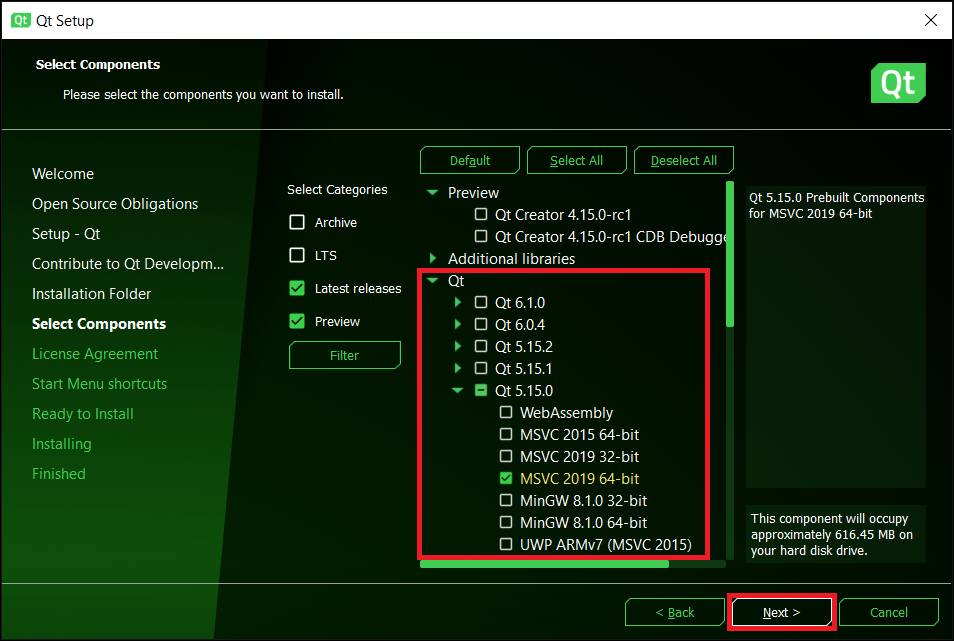
\includegraphics[width=12cm]{img/kap04_inst_sel}
	\caption{\uv{Select Components} časť Qt Setupu}
	\label{obr:kap4:inst_sel}
\end{figure}

\item Ďalej nasledujú bežné kroky pomocou ktorých dokončíme inštaláciu.

\end{itemize}

\subsection{Visual Studio 2019 a Qt}
\label{kap4:sec:VS2019_qt}
Teraz si ešte ukážeme integrovanie Visual studia 2019 spolu s Qt. Budeme si potrebovať nainštalovať \textit{Qt VS Tools}. Podrobný postup si ukážeme v nasledujúcich krokoch:
\begin{itemize}
\label{kap4:qt_vs_integ}
\item Priamo vo Visual Studiu si cez možnosť \textit{Extensions}$\rightarrow$\textit{Manage Extensions} do online hľadania zadáme \uv{Qt} a stiahneme si rozšírenie \uv{Qt Visual Studio Tools}~\cite{qt_vs_tools}
\item\label{kap4:qt_vs_integ:krok2} Po úspešnej inštalácii si musíme ešte vybrať Qt verziu cez možnosť \textit{Extensions}$\rightarrow$\textit{Qt VS Tools}$\rightarrow$\textit{Qt Versions} (ukázané na obrázku~\ref{obr:kap4:vs_versions}).

\begin{figure}[!htb]
	\centering
	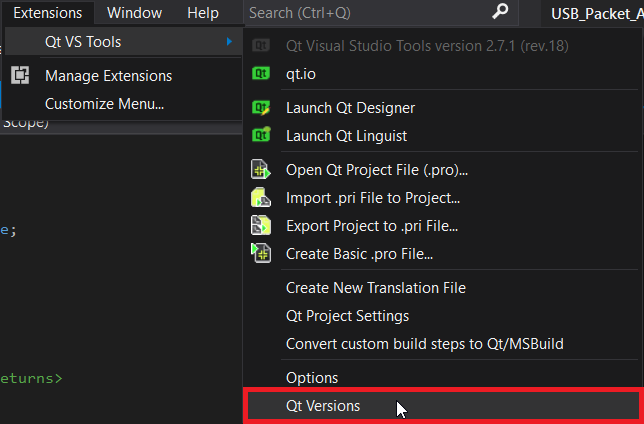
\includegraphics[width=12cm]{img/kap04_vs_versions}
	\caption{Visual Studio možnosť vybratia Qt verzie.}
	\label{obr:kap4:vs_versions}
\end{figure}

\item V dialógu sa teraz cez ikonu v stĺpčeku \uv{Path} (obrázok~\ref{obr:kap4:vs_path}) odkážeme do adresáru, kde sme nainštalovali \textit{Qt} a následne do adresáru \textit{5.15.0\/msvc2019\_64\/bin} kde máme nainštalovaný \textit{qmake.exe}.

\begin{figure}[!htb]
	\centering
	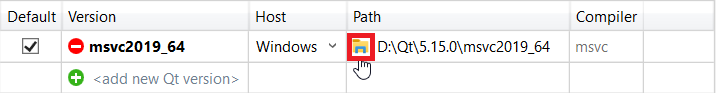
\includegraphics[width=12cm]{img/kap04_vs_path}
	\caption{Visual Studio zvolenie adresára ku \textit{qmake.exe}.}
	\label{obr:kap4:vs_path}
\end{figure}

\item Ako posledné si ešte skontrolujeme cez možnosť \textit{Project}$\rightarrow$\textit{Properties} v \textit{Configuration Properties}$\rightarrow$\textit{General} skontrolujeme, že máme nastavený \textit{C++ Language Standard} na možnosť \textit{ISO C++ 17} a \textit{Windows SDK Version} na verziu \textit{10.0.19041.0} ako na obrázku~\ref{obr:kap4:vs_prop}.

\begin{figure}[!htb]
	\centering
	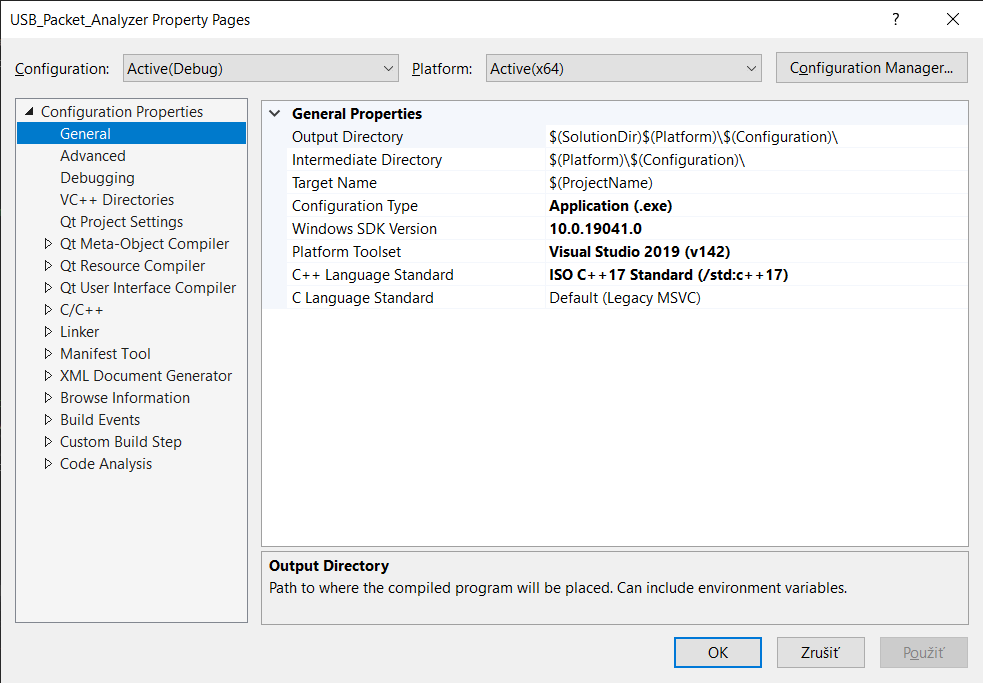
\includegraphics[width=12cm]{img/kap04_vs_prop}
	\caption{Visual Studio obecné nastavenia projektu.}
	\label{obr:kap4:vs_prop}
\end{figure}

\end{itemize}

Môže sa stať, že narazíme na bug keď nám krok~\ref{kap4:qt_vs_integ:krok2} nenastaví Qt verziu a nebudeme vedieť projekt preložiť kvôli errorom typu \uv{cannot open source file qbytearray}. V takom prípade prejdeme do možnosti \textit{Project}$\rightarrow$\textit{Properties}$\rightarrow$\textit{Qt~Project~Settings} a manuálne nastavíme \textit{Qt Installation} na \textit{msvc2019\_64} (obrázok~\ref{obr:kap4:vs_manual}).

\begin{figure}[!htb]
	\centering
	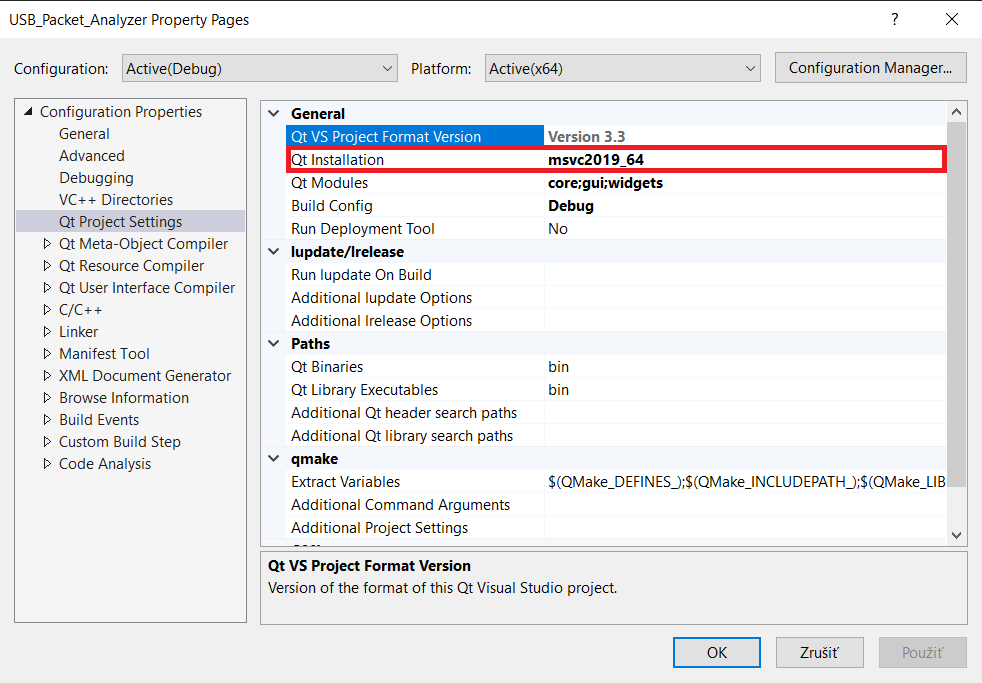
\includegraphics[width=12cm]{img/kap04_vs_manual}
	\caption{Visual Studio manuálne nastavenie Qt Installation.}
	\label{obr:kap4:vs_manual}
\end{figure}

V tomto momente by sme mali byť schopní úspešne skompilovať a spustiť náš program.

\newpage

\section{Architektúra aplikácie}

\begin{figure}[!htb]
	\centering
	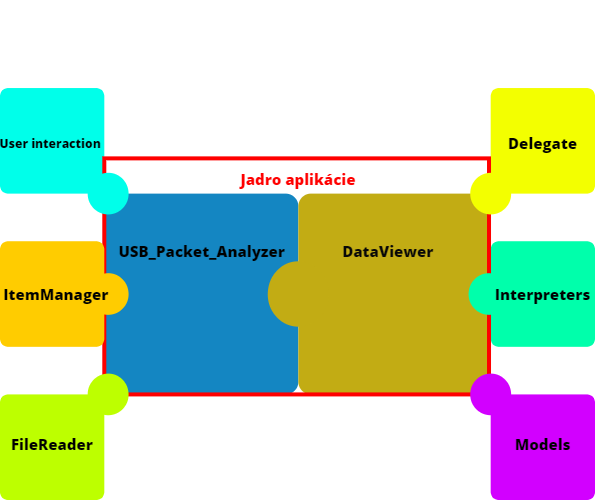
\includegraphics[width=\textwidth]{img/kap04_architektura}
	\caption{Diagram architektúry aplikácie}
	\label{obr:kap4:architek}
\end{figure}

V tejto sekcii si prejdeme celkovú stavbu aplikácie a akým spôsobom sú jednotlivé komponenty prepojené. Ako vidíme na obrázku~\ref{obr:kap4:architek}, aplikáciu môžeme rozdeliť do dvoch hlavných komponent, ktoré tvoria logické jadro programu: \texttt{USB\_Packet\_Analyzer} a \texttt{DataViewer}, na ktoré sa viažu ďalšie komponenty a dopĺňajú ich funkcionalitu. Teraz si podrobnejšie opíšeme obe hlavné komponenty spolu s komponentami, ktoré sú na nich napojené.

\section{USB\_Packet\_Analyzer}

USB\_Packet\_Analyzer tvorí hlavnú triedu programu, ktorá reprezentuje okno zobrazené užívateľovi hneď po zapnutí aplikácie. Naše hlavné okno pozostáva z nasledujúcich komponent:
\begin{itemize}
\item QTableWidget -- slúži na vyobrazenie základných informácií o paketoch.
\item 2 QRadioButtony -- slúžia na výber medzi analýzou fixného súboru (file capture), alebo súboru do ktorého môže sniffer počas analýzy niečo pripísať (live capture).
\item QCheckBox -- slúži na výber, či užívateľ chce farebne zvýrazniť detailnejší význam analyzovaných paketov alebo nie.
\item QLabel -- slúži na vyobrazenie názvu súboru, ktorý sa aktuálne spracováva.
\item QProgressBar -- progress bar ukazujúci stav spracovania súboru počas file capture.
\item 5 QPushButtonov -- tlačidlá, ktorých jednotlivú funkcionalitu si vysvetlíme nižšie v tejto sekcii~\ref{kap04:sec:open_button}.
\end{itemize}
Zároveň implementuje funkcie spojené s užívateľskou interakciou, od ktorej sa následne odvíja ďalšie správanie aplikácie.

\subsection{Užívateľská interakcia}
Ako sme už spomínali vyššie v kapitole~\ref{kap3:sec:model_view}, Qt využíva na komunikáciu medzi objektami tzv. \uv{Signals \& Slots}~\cite{signal_slot} mechanizmus, ktorý funguje ako alternatíva ku callback funkciám v iných frameworkoch. Qt widgety majú veľa preddefinovaných signálov (ku ktorým si môžeme dodefinovať ďalšie), ktoré sú emitované pri konkrétnom evente (napríklad QPushButton~\cite{qpushbutton} má signál \texttt{clicked()} ktorý je emitnutý pokiaľ je dané tlačidlo stlačené). Slot je funkcia, ktorá je zavolaná ako odpoveď na konkrétny signál. Prepojenie signálu so slotom prebieha pomocou metódy \texttt{QObject::connect(QObject* sender, signal, QObject* receiver, method)}, kde postupne definujeme inštanciu QObject spolu s jej konkrétnym signálom a následne inštanciu QObject spolu s jej metódou, ktorá sa má zavolať po emitovaní daného singálu. Qt má takisto možnosť \uv{Auto-Connect}~\cite{qt_autoconnect} pri ktorej stačí, že sa budeme držať štandardných konvencií a tým pádom nebudeme musieť manuálne prepájať jednotlivé signály a sloty pomocou \texttt{connect()} metódy. Toto využívame napríklad pri tlačidlách, konkrétne so signálom \texttt{clicked()}, kde stačí ak si vytvoríme slot pomocou nasledujúcej mennej konvencie: \texttt{void on\_\textless object name \textgreater\_clicked()}.

\begin{figure}[!htb]
	\centering
	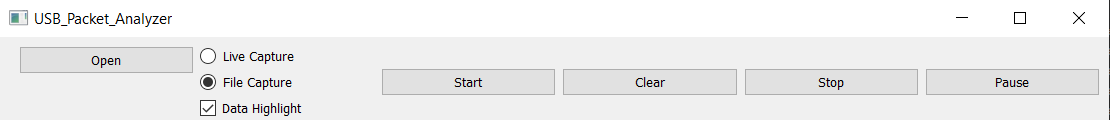
\includegraphics[width=\textwidth]{img/kap04_arch_buttons}
	\caption{Tlačidlá v aplikácii.}
	\label{obr:kap4:arch:buttons}
\end{figure}

Ako môžeme vidieť na obrázku~\ref{obr:kap4:arch:buttons}, naša aplikácia obsahuje hneď niekoľko tlačidieľ s odlišnou funkcionalitou o ktorú sa starajú už jednotlivé sloty, ktoré si teraz postupne opíšeme.

\paragraph{Open tlačidlo}
\label{kap04:sec:open_button}

slúži na vybratie si súboru na analýzu. To funguje na základe triedy QFileDialog~\cite{qfiledialog}, ktorá slúži na prechádzanie file systému. Užívateľovi sa zobrazí nový dialóg s intuitívnym ovládaním na ktoré je bežný užívateľ zvyknutý. Zároveň slúži na resetovanie progress baru a nastavenie labelu, ktorý zobrazuje aktuálne zvolený súbor.

\paragraph{Start tlačidlo}
\label{kap04:sec:start_button}

ako už napovedá jeho samotný názov, slúži na začatie analýzy. V tejto chvíli sa začne spracovávať súbor, ktorý si užívateľ zvolil pomocou predcházajúceho tlačidla Open~\ref{kap04:sec:open_button}. Spracovanie je následne vyobrazené pomocou QTableWidgetu, ktorým ako sme už riešili v kapitole~\ref{kap03:sec:zobr_zakl} vyobrazujeme základné informácie o jednotlivých paketoch. O cekové spracovanie súboru a jeho vyobrazenie tak ako aj o iné veci, sa stará trieda \textit{ItemManager}, o ktorej si povieme viac neskôr v sekcii~\ref{kap04:sec:item_manager}.

\paragraph{Clear tlačidlo}

zastáva funkciu vyčistenia plochy QTableWidgetu na ktorej sú vyobrazné základné informácie o paketoch. Takisto resetne progress bar, ktorým reprezentujeme v akom stave sa nachádzame z hľadiska spracovania daného súboru.

\paragraph{Stop tlačidlo}

spôsobí to, že sa úplne zastaví spracovávanie súboru. Využívané je pri analýze paketov v reálnom čase, čím stopne pridávanie nových paketov do QTableWidgetu. Akékoľvek ďalšie spracovávanie súborov už nie je umožnené. Ak by sme chceli analýzu len pozastaviť, tak v takom prípade použijeme tlačidlo Pause~\ref{kap04:sec:pause_button}.

\paragraph{Pause tlačidlo}
\label{kap04:sec:pause_button}

ako už bolo naznačené vyššie, slúži na pozastavenie analýzy. To znamená, že nové pakety nie sú pridávané do QTableWidgetu. Obnovenie analýzy je možné opätovným stlačením tlačidla (teraz už s nápisom \uv{Continue}), čím bude obnovené pridávanie nových paketov.

Z užívateľskej interakcie máme k dispozícii ešte jednu, o ktorej sme viac hovorili v kapitole~\ref{kap03:sec:zobr_zakl}, kde sme sa pre splnenie požiadavky na vyobrazenie detailnejších informácií o pakete na základe užívateľskej interakcie rozhodli pre dvojklik na položku reprezentujúcu daný paket.

\paragraph{\texttt{on\_tableWidget\_itemDoubleclicked(QTableWidget* item)}}
\label{kap04:sec:double_click}

je slot, ktorý sa volá po dvojkliku na konkrétny item v QTableWidget (pointer na daný item je poslaný ako parameter). V tejto metóde vytvoríme novú inštanciu triedy DataViewer s odpovedajúcimi parametrami a vyobrazíme jej dialógové okno, ktoré zobrazí detailnejšie informácie o danom pakete.

\subsection{ItemManager}
\label{kap04:sec:item_manager}
Interakciu užívateľa so systémom sme si už vysvetlili a teraz sa poďme pozrieť na samotné spracovávanie súborov. To má na starosti hlavne trieda ItemManager. Tá je implementovaná podľa návrhového vzoru singleton a vytvárame ju v konštruktore hlavnej triedy USB\_Packet\_Analyzer. Tento návrh nám okrem iného zároveň umožňuje počas analýzy v reálnom čase pokračovať v spracovávaní súboru na mieste, kde sme predtým skončili. V kapitole~\ref{kap03:sec:sprac_sub} sme sa rozhodli, že na čítanie súborov budeme používať QFile. ItemManager priamo so súborom, ale už len predparsovanými dátami v podobe jednotlivých paketov. Tie mu posiela inštancia triedy FileReader, ktorú má uloženú ako dátovú položku. FileReader má implementovanú celú logiku práce so súborom, pričom asi najpodstatnejšia je metóda \texttt{GetPacket()} -- prečíta zo súboru dáta, ktoré reprezentujú jeden paket a tie vráti zabaené v QByteArray.

\subsubsection{Selekcia paketov}

Ako sme už spomínali vyššie, samotná analýza začína stlačením tlačidla Start, kedy sa na inštancii ItemManagera zavolá metóda \texttt{ProcessFile(QString filename, bool liveReading)}. Ako nám už samotné názvy parametrov napovedajú, predávame v nej názov súboru, ktorý chceme spracovať a \texttt{bool} hodnotu určujúcu, či sa jedná o live capture alebo file capture. Táto metóda zaistí prostredníctvom FileReader inštancie otvorenie daného súboru a prečítanie jeho globálnej hlavičky. Ak sa jedná o live capture, nastaví timer aby kontroloval zmenu v súbore v pravidelných intervaloch 1 sekundy. Následne zavolá metódu \texttt{ProcessFileTillEnd(bool liveReading)}, ktorá pokračuje v spracovaní súboru od miesta kde čítanie naposledy skončilo, až po jeho koniec. Táto metóda je takisto spojená s \texttt{QTimer::timeout()} signálom, pre dodatočné spracovanie súboru v prípade pripísania nových paketov počas live capture. V tejto metóde si postupne od FileReaderu pýtame pomocou \texttt{GetPacket()} metódy dáta reprezentujúce jednotlivé pakety a tie posielame ako parameter funkcie \texttt{ProcessPacket(QByteArray)} na ich ďalšie spracovanie. Spracovanie samostatného paketu obsahuje niekoľko fáz:
\paragraph{Kontrola pre špeciálny typ paketu.}
\hfill \break
Pri spracovaní jednotlivých paketov riešime 2 nasledujúce veci:
\begin{itemize}
\item Dáta paketu reprezentujú Configuration Descriptor spolu s Interface/HID/Endpoint Descriptormi -- v takomto prípade bolo na zbernicu pripojené nové zariadenie a je potrebné si pre neho vytvoriť novú inštanciu typu BusDevice, o ktorej si viac povieme neskôr (ODKAZ).
\item Dáta paketu reprezentujú HID Report Descriptor -- v takom prípade je nutné daný Report Descriptor rozparsovať. Detailnejší opis si povieme nižšie v sekcii (ODKAZ).
\end{itemize}
Po týchto dvoch kontrolách a prípadne následných úkonoch, ktoré s nimi súvisia, posunieme dáta do metódy \texttt{FillUpItem(QByteArray)}.  

\paragraph{Rozdelenie dát do logických celkov.}
\hfill \break
Jej hlavná úloha je rozdeliť celý QByteArray na niekoľko menších podľa ich logického významu -- hlavička paketu, dodatočné dáta hlavičky a zvyšok poslaných dát. V kapitole~\ref{kap03:sec:uch_dat:qbytearray} sme sa rozhodli, že všetky tieto dáta zabalíme do QVariantu a uložíme do prvého QTableWidgetu na aktuálnom riadku. Ale ešte predtým ako dáta uložíme, si musíme celý riadok s odpovedajúcimi QTableWidgetami vytvoriť.

\paragraph{Pridanie jednotlivých riadkov.}
\hfill \break
Na to nám slúži metóda \texttt{InsertRow(PUSBPCAP\_BUFFER\_PACKET\_HEADER, unsigned char*)} -- prvý parameter je pointer na štruktúru reprezentujúcu hlavičku paketu, druhý parameter reprezentuje char* na dáta paketu. Pomocou tejto metódy teda vytvárame jednotlivé riadky v našej QTableWidget komponente. Po pridaní jednotlivých QTableWidgetItemov sa zavolaním metódy \texttt{ColorRow(PUSBPCAP\_BUFFER\_PACKET\_HEADER)} postará o farebné oddelenie jednotlivých riadkov podľa ich významu. Po úspešom pridaní riadku do QTableWidgetu a naplnení uložení jednotlivých dát do prvého QTableWidgetItemu sa vraciame späť do metódy \texttt{ProcessPacket(QByteArray)}, kde musíme urobiť ešte poslednú vec -- skontrolovať, či daný paket nereprezentuje Setup Paket pomocou metódy \texttt{CheckForSetupPacket(QByteArray)}. 

\paragraph{Kontrola na Setup Paket.}
\hfill \break
Ak sa jedná o Setup Paket, skontrolujeme položku bRequest. Ak má hodnotu GET\_DESCRIPTOR, znamená to, že USB host si od zariadenia vypýtal konkrétny typ desrcriptoru -- ten si vieme zistiť z položky wValue. V prípade, že sa jedná o Configuration Descriptor alebo HID Report Descriptor tak vieme, že dáta nasledujúceho paketu budú reprezentovať tento konkrétny descriptor a teda bude nutné ho podľa toho spracovať.
\hfill \break \newline
ItemManager obsahuje ešte jednu dôležitú metódu, a to \texttt{GetDataType(QTableWidgetItem*, QTableWidgetItem*)}, ktorá je schopná na základe dát, ktoré sme si uložili do konkrétneho QTableWidgetItemu zistiť presný typ prenosu. V prípade, že sa jedná o Control Transfer tak určuje aký typ descriptoru reprezentujú \uv{zvyškové dáta} paketu (dáta nasledujúce po hlavičke a po nepovinnej dodatočnej hlavičke). V danom prenose sa ale môže nachádzať aj viac descriptorov súčasne -- konkrétne je to v prípade ak zariadenie posiela svoj Configuration Descriptor spolu s Interface/Endpoint/HID descriptormi. V tomto prípade metóda vráti, že sa jedná o Configuration Descriptor.

Týmto sme si opísali akým spôsobom sa spracovávajú súbory, vyobrazujú sa základné informácie o paketoch a spôsob uloženia dát jednotlivých paketov. Teraz sa pozrieme ako je v našom programe riešená detailnejšia analýza (napírklad hexdump alebo sémantické vyobrazenie dát) konkrétnych paketov na základe informácií, ktoré sme si pri nich uložili.

\section{DataViewer}
Trieda reprezentujúca pop-up okno s detailnejšou analýzou konkrétneho paketu. Dané okno pozostáva z nasledujúcich komponent:
\begin{itemize}
\item 2 QTableView -- slúžia na vyobrazenie hexdumpu. Jeden pre hex časť a druhý pre tlačiteľné znaky.
\item 3 QTreeView -- každý slúži na vyobrazenie sémantického významu rozdielnych dát v podobe stromovej štruktúry. Jeden zobrazuje hlavičku paketu spolu s nepovinnou hlavičkou, ďalší vyobrazuje Color Map slúžiacu na lepšiu orentáciu v hexdumpe a posledný ukazuje zvyškové dáta -- napríklad význam rôznych descriptorov alebo inputu zariadenia.
\item 6 QLabelov -- slúžia na opis toho, čo je vyobrazené na predošlých komponentách. 
\end{itemize}

Ako sme sa si vysvetlili vyššie~\ref{kap04:sec:double_click}, nová inštancia DataVieweru sa vytvára v momente keď užívateľ dvojklikne na riadok reprezentujúci konkrétny paket. Do konštruktoru si predávame 3 základné veci:
\begin{enumerate}
\item Pointer na QTableWidgetItem, ktorý v sebe obsahuje dáta daného paketu.

\item Typ prenosu/descriptoru, ktorý získame pomocou vyššie sponínanej metódy \texttt{ItemManager::GetDataType(QTableWidgetItem*, QTableWidgetItem*)}.

\item Bool hodnotu, ktorá určuje či budeme dáta v hexdumpe farebne zvýrazňovať alebo nie. Túto hodnotu získame z QCheckBoxu hlavného okna.
\end{enumerate}

V konštruktore následne inicializujeme naše komponenty -- keďže využívame spôsob programovania pomocou Qt Model/View architektúry, inicializácia zahŕňa vytvorenie modelov a delegátov a ich následné priradenie k jednotlivým viewerom. Teraz si povieme obecný spôsob fungovania modelov a delegátov v Qt, a následne si priblížime implementáciu našich konkrétnych modelov.


\subsection{Model}
Model je v Qt obyčajná trieda založená na QAbstractItemModel~\cite{qabstractitemmodel} triede, ktorá spĺňa preddefinovaný interface vďaka ktorému viewery a delegáti pristupujú k dátam. Naše modely môžu byť takisto odvodené od viac špecifických modelov, ktoré poskytuje Qt ako napríklad QAbstractTableModel~\cite{qabstracttablemodel}. Nezáleží na tom akým spôsobom budú naše dáta uložené, modely ich reprezentujú ako hierarchickú štruktúru obsahujúcu tabuľku itemov. Prístup k položkám modelu je potom zaistený pomocou tzv. \uv{model indexov}. Viewery a delegáti používajú tieto indexy aby sa odkázali na konkrétne dáta, ktoré neskôr vyobrazujú. Aby sme získali index na konkrétne dáta, potrebujeme špecifikovať tri veci: číslo riadku, číslo stĺpca a model index rodičovského itemu.
\paragraph{Číslo riadku a číslo stĺpca:} Ako sme už spomínali, modely reprezentujú itemy pomocou tabuľkovej štruktúry. Pomocou čísla riadku a stĺpca sa odkážeme na konkrétny item v tabuľke.
\paragraph{Model index rodičovského itemu:}  Tabuľková štruktúra ponúka dobrú reprezentáciu v prípade tabuliek, avšak nie je úplne ideálna ak si dáta ukladáme a chceme ich vyobraziť v podobe stromovej štruktúry. V takejto štruktúre má prirodzene každý item (až na koreň stromu) rodiča a ľubovoľný počet synov. Na index konkrétneho vrcholu v strome nám tak bude stačiť poznať index jeho rodiča a ktorý syn v poradí to je (to môžeme reprezentovať číslom riadku).
Každý item v modeli má definovanú tzv. \uv{role}, ktorá určuje ako sa na dané dáta máme pozerať. Napríklad \textit{Qt::DisplayRole} označuje dáta, ktoré majú byť vo vieweri vyobrazené ako text


\subsection{Delegát}
\label{kap04:sec:delegate}
Delegáti obecne slúžia na vizualizáciu dát s možnosťou ich editácie. Štandardný interface pre delegátov je poskytnutý triedov QAbstractItemDelegate~\cite{qabstractitemdelegate}. Od delegátov sa predpokladá, že implementujú metódy \texttt{paint()} a \texttt{sizeHint()} na vyobrazenie kontentu.


\subsection{Hexdump}
Teraz sa pozrieme na konkrétny model pre naše komponenty reprezentujúce hexdump. Implementujeme ho vlastnou triedou \texttt{HexdumpModel}, ktorá je odvodená od \texttt{QAbstractTableModel}. V konštruktore si predávame nasledujúce:
\begin{enumerate}
\item \texttt{QTableWidgetItem* item} -- Pointer na item obsahujúci dáta konkrétneho paketu, ktoré budeme v hexdumpe vyobrazovať.

\item \texttt{bool hexView} -- Keďže máme rovnaký model pre hex časť a tlačiteľné znaky, potrebujeme vedieť rozlíšiť o ktorú z týchto dvoch možností sa jedná. Na to presne slúži táto bool hodnota.

\item \texttt{HeaderDataType additionalDataType} -- Typ prenosu/descriptoru dát paketu.

\item \texttt{QObject* parent} -- Pointer na DataViewer inštanciu.
\end{enumerate}

QAbstractTableModel ponúka viac špecializovaný interface ako QAbstractItemModel a podľa dokumentácie implementuje metódy \texttt{index()} a \texttt{parent()}. Nám ostáva implementovať metódy \texttt{columnCount()}, \texttt{rowCount()} a \texttt{data()}. Odporúčané je takisto implementovať metódu \texttt{headerData()}.

\paragraph{columnCount()} metóda vráti počet stĺpcov z ktorých bude pozostávať výsledný hexdump. V našom programe sme sa rozhodli zvoliť konštantnú hodnotu, ktorá je pre hexdump bežná -- 16.

\paragraph{rowCount()} metóda vráti počet riadkov, z ktorých bude pozostávať výsledný hexdump. Vzhľadom na to, že máme k dispozícii QTableWidgetItem obsahujúci všetky dáta, ktoré budeme chcieť vyobraziť v hexdumpe, stačí nám spočítať ich dĺžku a vydeliť ju počtom stĺpcov na jeden riadok (pričom z výsledku berieme hornú celú časť).

\paragraph{data()} metóda vracia QVariant reprezentujúci konkrétny item v hexdumpe. Ten pozostáva z dvojice:
\begin{enumerate}
\item Konkrétne dáta, ktoré budú vyobrazené -- 1B buď v hex tvare, alebo v tvare tlačiteľného znaku
\item \texttt{HeaderDataType} položka určujúca presný typ prenosu/descriptoru. Podľa tejto položky budeme následne určovať akou farbou bude daný item v hexdumpe označený. Nemôžeme tu ale iba skopírovať položku, ktorú sme dostali ako parameter v konštruktore, pretože hodnota tejto položky pochádza z metódy \texttt{ItemManager::GetDataType} a ako sme už spomínali, tá nevie rozoznať rozdiel medzi jednotlivými descriptormi pokiaľ sú poslané v jednom prenose. My ale chceme vedieť farebne odlíšiť aj descriptory, ktoré zariadenie poslalo v jednom prenose. Konkrétnu hodnotu teda zistíme pomocou metódy \texttt{GetDataRepresentationType} v ktorej pokiaľ sa jedná o Configuration Descriptor, prejdeme zvyškové dáta paketu a na základe indexu v ktorej časti sa nachádzame presne určíme typ descriptoru.
\end{enumerate}

\paragraph{headerData()} metóda nám umožňuje nastaviť vertikálnu hlavičku na ktorú je užívateľ pri bežnom hexdumpe zvyknutý -- offset bytov v hexadecimálnej reprezentácii.


\subsection{Hexdump delegát}
Delegát pre hexdump je naša trieda \texttt{HexdumpDelegate} odvodená od triedy QStyledItemDelegate. Tento delegát slúži na vyobrazenie jednotlivých položiek v hexdumpe, tak ako aj ich farebné zvýraznenie. Pri vytváraní inštancie daného delegátu jej nastavíme bool parameter \textit{dataHighlight} určujúci, či máme farebne zvýrazňovať dáta v hexdumpe. Ako sme už naznačili vyššie v sekcii~\ref{kap04:sec:delegate}, musíme implementovať metódy \texttt{paint()} a \texttt{sizeHint()}.

\paragraph{paint()} metóda dostane ako parameter model index z ktorého získa dvojicu dát QVariant, ktorú sme vytvorili pomocou nášho hexdump modelu v metóde \texttt{data()}. Podľa dátovej položky \textit{dataHighlight} sa určí, či budeme farbne zvýrazňovať daný item -- ak áno, z druhej položky QVariantu získaného z model indexu zistíme presný typ prenosu/descriptoru (teraz už aj v prípade, že bolo poslaných viac descriptorov v jednom prenose) a na základe toho zafarbíme daný item.

\paragraph{sizeHint()} metódou vrátime konštantnú hodnotu \texttt{QSize(30,30)} ktorá určuje veľkosť bunky hexdumpu.


Teraz keď sme si vysvetlili fungovanie HexdumpModelu a HexdumpDelegatu, stačí ak ich nastavíme danému QTableVieweru. To urobíme pomocou metódy \texttt{setModel()} a \texttt{setItemDelegate()}.

Momentálne nám ostávajú ešte modely pre 3 komponenty reprezentujúce Color Map, hlavička paketu a zvyškové dáta. Všetky majú viewer typu QTreeView, takže k nim budeme potrebovať model prispôsobený na stromovú štruktúru. Každá komponenta má vlastný model, niektorú funkcionalitu ale majú spoločnú a preto sme si vytvorili triedu \texttt{TreeItemBaseModel}, ktorá dedí od triedy \texttt{QAbstractItemModel}. Každý z modelov pre jednotlivé QTreeViewery bude následne dediť od \texttt{TreeItemBaseModel}. Musíme ešte vyriešiť spôsob reprezentácie tejto stromovej štruktúry. Na to nám poslúži naša trieda \texttt{TreeItem}. Pri implementácii tried TreeItemBaseModel a TreeItem sme sa inšpirovali príkladom z Qt dokumentácie~\cite{qtreemodelexample}.

\subsection{TreeItem}
\label{kap04:sec:tree_item}
Reprezentuje jeden vrchol v stromovej štruktúre. Uchováva si v sebe nasledovné:
\begin{itemize}
\item \texttt{TreeItem* parent} -- pointer na svojho rodiča.
\item \texttt{QVector\textless~std::shared\_ptr\textless~TreeItem\textgreater\textgreater childs} -- list svojich synov
\item \texttt{QVector\textless~QVariant\textgreater} data -- dáta, ktoré budú následne vyobrazené v QTreeView. Viewer samotný ponúka možnosť viacerých stĺpcov v jednom iteme a preto si dáta ukladáme v QVectore. Každá položka QVariant vo vectore tak rerezentuje dáta v jednotlivých stĺpcoch.
\end{itemize} 

Následne tu máme implemtované bežné funkcie potrebné pre prácu so stromovou štruktúrov ako napríklad \texttt{ChildCount()}, \texttt{AppendChild()} alebo \texttt{ColumnCount()}, ktorých význam a princíp fungovania je bližšie opísaný v zdrojvých kódoch v súboroch \textit{TreeItem.hpp} a \text{TreeItem.cpp}, ktoré boli poskytnuté ako príloha k tejto práci.
Trochu podstatnejší je konštruktor, ktorý vyzerá nasledovne:
\texttt{TreeItem(QVector\textless~QVariant\textgreater) data\_, TreeItem* parent\_} -- ako parameter dostávame dáta, ktoré si bude daný vrchol držať a pointer na svojho rodiča. V prípade že sa jedná o koreň stromu bude rodič nastavený na \texttt{nullptr}.



\subsection{TreeItemBaseModel}
Poskytuje spoločný interface pre modely fungujúcimi pre stromové štruktúry. Takisto v sebe drží \texttt{std::unique\_ptr\textless~TreeItem\textgreater rootItem} reprezentujúci koreň stromu.  Ako spoločný predok všetkých modelov pre stromové štruktúry má implementované metódy, ktorých funkcionalita sa v odvodených triedach nemení a patria medzi ne:
\begin{itemize}
\item \texttt{index()} -- vytvorí a vráti QModelIndex na základe parametrov (číslo riadku, číslo stĺpca a model index rodičovského itemu).
\item \texttt{parent()} -- na základe parametru QModelIndex vráti index rodiča daného vrcholu. Ak sa jedná o koreň stromu, podľa konvencie vrátime QModelIndex().
\item \texttt{rowCount()} -- vráti počet synov vrcholu.
\item \texttt{columnCount()} -- vráti počet stĺpcov dát vrcholu.
\end{itemize}
 
 Následne tu máme ešte implementované metódy, ktoré sa nám hodia pri vyobrazovaní dát v QTreeView ale nie sú súčasťou QAbstractItemModelu:
\begin{itemize}
\item \texttt{CharToHexConvert(char** addr, int len, QString\& data)} -- v parametri \textit{data} vráti hex reprezentáciu prvých \textit{len} znakov char poľa uloženého na adrese \textit{addr}.
\item \texttt{ShowBits\textless~T\textgreater(uint32\_t start, size\_t size, T number)}  -- parametrizovaná funckia, ktorá bola vytvorená pre účel splnenia požiadavky~\ref{uvod:poz:show_bits} na vyobrazenie významu dát až na úrovni jednotlivých bitov. Výsledok zapisujeme do QStringu, ktorý na konci vrátime. Ako parameter T dostaneme číslo, ktorého bity budeme chcieť ukázať. To prechádzame postupne bit po bite a v momente keď sa nachádzame v intervale \textless~start, start + size) zapisujeme do QStringu hodnoty jednotlivých bitov. Ak sa nachádzame mimo intervalu, zapisujeme \uv{.}.
\end{itemize}

TreeItemBaseModel obsahuje ešte tzv. \uv{pure virtual} funkcie \texttt{data()} a \texttt{headerData()}, ktorých implementácia sa bude líšiť na základe dedenej triedy -- je teda ich povinnosťou tieto metódy implementovať.


\subsection{ColorMapModel}
ColorMapModel je naša trieda odvodená od TreeItemBaseModel reprezentujúca model pre Color Map. Ako sme už vyššie spomínali, musí implementovať 2 funkcie: \texttt{headerData()} a \texttt{data()}. Ešte predtým si ale musíme rozmyslieť odkiaľ zoberieme dáta, ktoré budeme chcieť v Color Mape zobrazovať. Vyššie sme si spomínali triedu \texttt{TreeItem}~\ref{kap04:sec:tree_item}, ktorá reprezentuje jeden vrchol v stromovej štruktúre, ktorá si bude udržiavať naše dáta. Celý strom si musíme najprv vytvoriť a naplniť ho dátami, a o to sa stará funkcia \texttt{SetupModelData()}.

\paragraph{SetupModelData()} je metóda, ktorú voláme priamo v konštruktore ColorMapModel. Keďže dedíme od triedy TreeItemBaseModel, máme k dispozícii koreň stromu (\texttt{std::unique\_ptr\textless~TreeItem\textgreater rootItem}) pomocou ktorého budeme cez TreeItem metódy budovať strom. Dáta každého vrcholu budú pozostávať z 2 položiek:
\begin{itemize}
\item \texttt{HeaderDataType} -- položka určujúca presný typ prenosu/descriptoru. Vďaka tejto položke budeme schopní priradiť odpovedajúcu farbu každému itemu v QTreeView.
\item string reprezentujúci názov typu prenosu/descriptoru.
\end{itemize}

ColorMapModel obsahuje ešte jednu špecifickú metódu \texttt{GetDataTypeColor(HeaderDataType dataType)}, ktorá na základe parametru type vráti jemu odpovedajúcu farbu. Farby ku každému HeaderDataType máme nadefinované v triede DataHolder o ktorej si povieme viac nižšie (ODKAZ). Teraz si prejdeme implementáciu už spomínaných virtuálnych funkcií:
\begin{itemize}
\item \texttt{headerData()} -- keďže v Color Map nechceme mať žiadnu hlavičku, funkcia vracia prázdny QVariant().
\item \texttt{data(QModelIndex\& index, int role)} -- podľa parametru role zistíme o aké dáta sa jedná. Ak sa role rovná \textit{Qt::DecorationRole}, vrátime farbu pomocou metódy GetDataTypeColor(). Ak sa role rovná \textit{Qt::DisplayRole}, vrátime textovú reprezentáciu typu prenosu/descriptoru, ktorú sme si uložili do itemu ako druhú položku. Ak sa role rovná hocičomu inému, vrátime prázdny QVariant().
\end{itemize}


\subsection{USBPCapHeaderModel}
je trieda odvodená od TreeItemBaseModel a reprezentuje model pre QTreeView, ktorý vyobrazuje detailnejšie informácie hlavičky paketu. V tejto triede máme takisto metódu \texttt{SetupModelData()}, ktorá vytvorí stromovú štruktúru reprezentujúcu hlavičku paketu. Hlavička paketu má fixný formát určený štruktúrou \texttt{USBPCAP\_BUFFER\_PACKET\_HEADER}, ktorú definuje sniffer USBPcap cez ktorý zachytávame pakety na zbernici.
Virtuálne funkcie sú implementované nasledovne:
\begin{itemize}
\label{kap04:sec:usbh_virt}
\item \texttt{headerData(int section, Qt::Orientation orientation, int role)} -- dáta hlavičky si typicky budeme ukladať do QVectoru \textit{data} nášho rootItemu. Podľa parametru orientation zistíme o akú hlavičku sa jedná (vertikálnu/horizontálnu). Keďže v našom QTreeView chceme mať horizontálnu hlavičku, testujeme na zhodu práve s Qt::Horizontal hodnotou a zároveň kontrolujeme či sa role rovná Qt::DisplayRole. Následne už len vrátime dáta zo stĺpca, ktorý je definovaný parametrom section.
\item \texttt{data(QModelIndex\& index, int role)} -- pokiaľ sa role nerovná Qt::DisplayRole alebo index nie je validný, vrátime prázdny QVariant(). V opačnom prípade is pomocou indexu získame pointer na daný item a vrátime dáta z konkrétneho stĺpca (hodnotu stĺpca zistíme takisto z indexu).
\end{itemize}

\subsection{AdditionalDataModel}
je trieda, ktorá je takisto odvodená od TreeItemBaseModel a reprezentuje model zvyškových dát paketu. To zahŕňa napríklad dáte reprezentujúce rôzne typy descriptorov, input zariadení atď. Virtuálne metódy \texttt{data()} a \texttt{headerData} riešime rovnakým spôsobom ako pri USBPCapHeaderModel~\ref{kap04:sec:usbh_virt}. Problém nastáva až vo funkcii, ktorá má vytvoriť stromovú štruktúru. V minulých modeloch sme totiž presne vedeli čo majú jednotlivé dáta reprezentovať a ako bude vyzerať im odpovedajúci strom. Teraz to ale nie je také jednoduché, pretože zvyškové dáta paketu môžu mať rozličnú reprezentáciu, ktorá je určená až za runtimu. (odkaz na cieľ s ľahkou rozsiritelnostou ?) Preto túto situáciu vyriešime pomocou známeho návrhového vzoru -- factory. Zadefinujeme si triedy, ktorých jediná úloha bude vytvoriť špecifickú stromovú štruktúru odpovedajúcu danému typu dát. Tieto triedy budeme obecne nazývať \uv{interpretery}.

\subsection{BaseInterpreter}




%Budeme si potrebovať nainštalovať Qt pre Windows. podla videa, verzia 5.15.0 len msvc 2019 64bit. inak ostatne default. zatial som este nainstaloval QT VS extension. teraz idem updatenut SDK na verziu 10.0.19041.0 -- to vymazalo errory typu ''cannot open source file cctype'' , teraz mi este ostali ''cannot open source file qbytearray'' a podobne spojene cisto s qt : pravdepodobne bug. musel som ist manualne do Project->properties->Qt Project SEttings a nastavit Qt installation na verziu 5.15.0_msvc2019_64. A UZ TO BEZIIII :)



























\newpage
\section{Architekrúra aplikácie}
\section{Jadro aplikácie}
\subsection{USB\_Packet\_Analyzer}
riadi celkovy beh programu, reaguje na input od uzivatela
\subsection{Item Manager}
spracovanie samostatneho packetu a ulozenie dat o nom
\subsection{DataViewer}
trieda ktora ma na starosti vyskakovacie okno po dvojkliku a item a nasledne reaguje na input od uzivatela v okne
\subsection{TreeItem}
reprezentuje jednotlive nody v stromovej strukture ktora sa potom vyuziva na zobrazenie dat v QTreeView
\section{Modely}
\subsection{AdditionaldataModel}
model na spravovanie zvysnych dat(data ktore nie su sucastou hlavicky packetu)
\subsection{ColorMapModel}
vyobrazenie pomocnej mapy na lepsie sa zorientovanie v zvyraznemom hexdumpe
\subsection{DataViewerModel}
model na hexdump - prenasa hex/printable a zaroven o co vlastne ide(konkretny descriptor, interrupt data, ...)
\subsection{TreeItemBaseModel}
model na QTreeView ktorz vyuziva TreeItem
\subsection{USBPcapHeaderModel}
model na QTreeView ale specialne pre USBPcap hlavicku packetu
\section{Interpretery}
\subsection{BaseInterpreter}
abstractna trieda od ktorej dedia vsetkz interpretery
\subsection{Interpreter factory}
facory trieda na pridelenie konkretneho interpreteru za runtimu kvoli jednoduchosti na lepsie rozsirenie programu do buducnosti
\subsection{Interpretery descriptorov}
Config,Device,Setup,String,...
\subsection{Interrupt transfer interpretery}
obecne interrupt transfer interpreter - sluzi skor ako factory na rozne doteraz implementovane HID zariadenia
\subsubsection{Joystick interpreter}
\subsubsection{Mouse interpreter}
\subsubsection{Keyboard interpreter}
\section{Delegáti}
\subsubsection{DataViewerDelegate}
Qt delegat - stara sa o highlight hexdumpu
\section{HID}
\subsection{HIDDevices}
staticka trieda, drzi vsetky rozpoznane HID zariadenia a obsahuje funkcie specificke nich - parsovanie HID Report descriptoru
\section{Práca so súbormi}
\subsection{FileReader}
praca zo suborom a predavanie precitanych dat, offline/online capture, QFile vs std::istream
\section{Globálne dáta}
\subsection{ConstDataHolder}
staticka trieda na drzanie si konstant ktore su potrebne napriec celym programom. Mapovanie z enumu do jeho stringovej reprezentacie
\subsection{PacketExternStructs}
obsahuje definiciu vsetkych dolezitych USBPcap structov, pcap structov, enumov a vsetkych structov ktore pouzivam v aplikacii












\chapter{Možnosti rozšírenia}
V tejto kapitole sa pozrieme na rôzne možnosti a smery, akými by sme mohli našu aplikáciu ďalej rozšíriť.
\section{Ukladanie výstupu do súboru}
Niektoré analyzátory ponúkajú ukladanie výpisu do rôznych súborov. V prípade ak by sme sa rozhodli našu aplikáciu rozšíriť o možnosť ukladania analýzy do súboru, museli by sme si rozmyslieť niekoľko nasledujúcich vecí:

\paragraph{Formát výpisu}
\hfill \break
Akým spôsobom bude vyzerať výstup analýzy. Na výber máme viacero možností od obyčajného textového výstupu až po obrázky alebo rôzne tabuľky. Na začiatok by nebolo príliš zložité zaintegrovať výpis analýzy v textovom formáte. Všetky dáta máme interne reprezentované v podobe QByteArray alebo stromovej štruktúry, ktoré je možné jednoducho prechádzať. Samozrejme musíme myslieť na to, že textový výpis nie je tak flexibilný a interaktívny ako prípadný QTreeView, takže vyobrazenie stromovej štruktúry by pravdepodobne nevyzeralo ideálne.

\paragraph{Rozhodnutie užívateľa, či bude danú analýzu ukladať do súboru alebo nie}
\hfill \break
Musíme myslieť na to, v akej fáze programu umožníme užívateľovi sa najneskôr rozhodnúť o ukladaní danej analýzy do súboru. Momentálne si všetky dáta uchovávame v samostatných QTableWidgetItemoch uložených v QTableWidgete hlavného okna aplikácie. Užívateľ má ale možnosť toto okno \uv{vyčistiť} pomocou tlačidla Clear~\ref{kap04:sec:clear_button}, ktoré vymaže všetky QTableWidgetItemy a tým pádom stratíme referenciu na všetky dáta, ktoré v sebe dané itemy uchovávajú. Doteraz sme sa tým nemuseli zaoberať, pretože dané dáta sem potrebovali na analýzu paketov reprezentovaných riadkom v QTableWidgete, takže akonáhle bol riadok vymazaný pomocu Clear tlačidla, detailnejšia analýza daného paketu už nebola možná. Niektoré možné riešenia tohto problému by mohli byť nasledujúce:
\begin{itemize}
\item V prípade, že umožníme užívateľovi si uložiť analýzu do súboru len do momentu pokiaľ nestlačí tlačidlo Start, máme na výber prakticky 2 možnosti:
\begin{enumerate}
\item \label{kap05:sec:refer} Ukladať si referencie na jednotlivé QTableWidgetItemy až do momentu skončenia programu, kedy jednorázovo zapíšeme do súboru celú analýzu.
\item \label{kap05:sec:priebez} Priebežne zapisovať do súboru analýzu jednotlivých paketov.
\end{enumerate}
Riešenie~\ref{kap05:sec:refer} prináša tú nevýhodu, že si musíme držať v pamäti všetky dáta paketov a zároveň by ukončenie aplikácie trvalo dlhšiu dobu, pretože by sa musela postupne vykonať a zapísať detailná analýza každého paketu. Naopak riešenie~\ref{kap05:sec:priebez} nás zbavuje oboch týchto problémov, ale mohla by mať nepriaznivý dopad na užívateľskú interakciu s aplikáciou, pretože v pozadí by prebiehal proces zapisovania a analýzy. To by sa samozrejme dalo optimalizovať rôznymi spôsobmi -- zapisovať len v momente pokiaľ užívateľ neinteraguje s aplikáciou, využiť metódy paralelného programovania a na zápis/analýzu použiť viac vláken, atď.

\item V prípade, že umožníme užívateľovi rozhodnúť o zápise do súboru hocikedy v priebehu používania aplikácie, musíme mať dáta jednotlivých paketov k dispozícii aj po ich odstráneni z QTableWidgetu tlačidlom Clear. Ako toho dosiahnuť sme naznačili vyššie v riešení~\ref{kap05:sec:refer} spolu s jeho nevýhodami.
\end{itemize}

Dôležité je ale spomenúť, že pridaním ukladania výpisu do súboru nijakým vážnym spôsobom nezasahujeme do programu a nemodifikujeme už naimplementované časti. Všetky dáta máme v aplikácii pripravené a jediné čo nám ostáva vyriešiť je ich spracovanie do súboru.

\section{Iná vizuálna reprezentácia dát}
Momentálne vyobrazujeme dáta za pomoci viewerov -- QTableView, QTreeView. Ako sme si už spomínali vyššie, celé to prebieha na základe Model/View architektúry, ktorá nám umožnuje od seba oddeliť dáta a spôsob akým ich vyobrazujeme. Na základe toho by pre nás nemalo byť tak náročné implementovať nové spôsoby vizuálnej reprezentácie dát. To by sme vedeli dosiahnuť pridaním nového typu vieweru. Mohli by sme si vybrať z už existujúcich, alebo si kľudne naimplementovať vlastný, ktorý by odpovedal našim predstavám vyobrazenia dát. Momentálne máme vytvorených viacero modelov pre špecifické časti našich dát (HexdumpModel pre všetky dáta paketu na vyobrazenie hexdumpu, USBPCapHeaderModel pre hlavičku paketu na jej vyobrazenie pomocou stromovej štruktúry, atď.). Všetky tieto modely sme implementovali z dôvodu aby sme jednoducho vedeli vyobraziť dáta v jednotlivých vieweroch. Preto by pridanie nového vieweru malo pravdepodobne za následok nutnosť implementovať aj tomu odpovedajúci model.

Zaujímavý spôsob vyobrazenia dát by bolo napríklad pomocou koláčového grafu. Vedeli by sme tak vizuálne zobraziť pomer rôznych dát ako napríklad:
\begin{itemize}
\item pomer rôznych typov prenosov (Control/Interrupt/Bulk/Isochronous) počas zachytávania paketov.
\item pomer veľkosti dát hlavičky paketu a zvyškových dát.
\item pomer veľkosti dát poslaných zariadením a USB hostom.
\item pomer zvyškových dát v paketoch vzhľadom na typ prenosu.
\end{itemize}

Takisto by mohlo byť zaujímavé vyobraziť dáta viac grafickým spôsobom, napríklad ako je ukázané na obrázku~\ref{obr:kap5:graphics_packets} nižšie.

\begin{figure}[!htb]
	\centering
	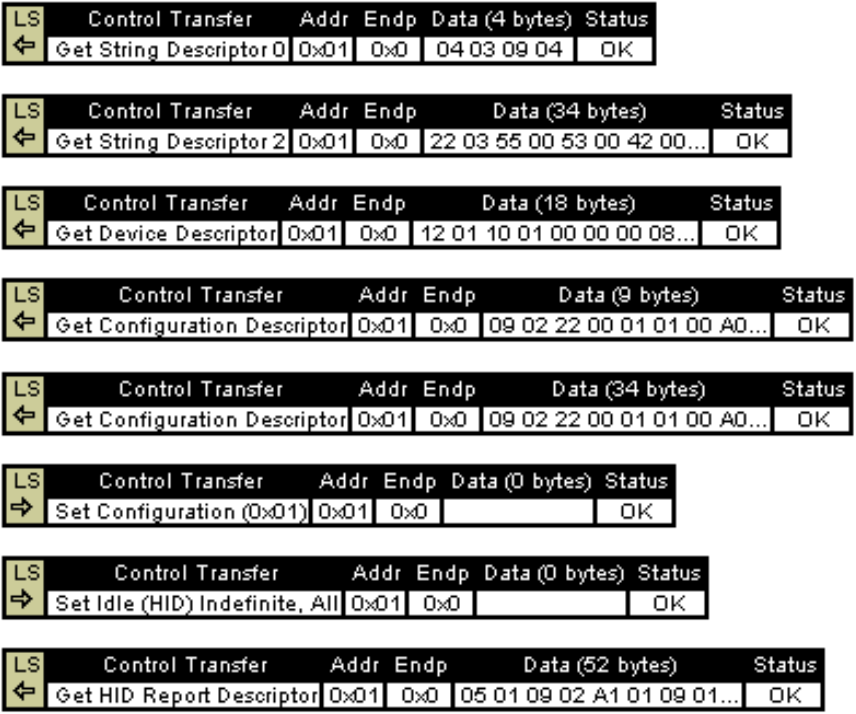
\includegraphics[width=12cm]{img/kap05_graphics_packets}
	\caption{Ukážka grafického vyobrazenia paketov. Obrázok prevzatý zo stránky USB Made Simple~\cite{usbmadesimple_graphics}}
	\label{obr:kap5:graphics_packets}
\end{figure}

\newpage
\section{Pridávanie nových Interpreterov pre descriptory}
Vrámci rozšírenia programu by sme mohli chcieť pridať analýzu pre nové descriptory. V takomto prípade musíme vyriešiť nasledujúce:
\begin{itemize}
\item Definícia descriptoru -- musíme si rozmyslieť odkiaľ zoženieme definíciu daného descriptoru. Môžeme si ho buď nadefinovať sami alebo použiť stávajúce definície z rôznych knižníc. Momentálne si sami definujeme len jeden descriptor -- HID Descriptor a všetky ostatné descriptory ktorých analýzu podporujeme sú definované v súbore usbspec.h.
\item Aby sme vedeli v programe tento druh descriptoru rozpoznať, musíme si pridať jeho číselnú reprezentáciu do enumov:
\begin{enumerate}
\item \textit{HeaderDataType} -- umožní novú položku v \textit{InterpreterFactory}.
\item \textit{DesriptorTypes} -- umožní rozpoznanie daného descriptoru z údajov Setup Paketu. Táto hodnota sa bude musieť presne zhodovať s hodnotou descriptoru definovanou USB špecifikáciou.
\end{enumerate}
\item Definovať v metóde \texttt{ItemManager::GetDataType()} prevod z \textit{DescriptorTypes} enumu na enum \text{HeaderDataType}.
\item Naimplementovať nový Interpreter pre daný descriptor.
\item Pridať do \textit{InterpreterFactory} možnosť vytvorenia Interpreteru pre daný descriptor.
\end{itemize}
\section{Pridanie Intepreteru pre Interrupt Transfer}
O analýzu zariadení, ktoré svoje dáta posielajú cez Interrupt Transfer sa momentálne stará \textit{InterruptTransferInterpreter}, ktorý pôsobí skôr ako ďalšia factory než ako samotný interpreter. Pre pridanie nového zariadenia by sme sa museli postarať o nasledujúce:
\begin{itemize}
\item Číselne zareprezentovať dané zariadenie pridaním novej položky do \textit{SupportedDevices} enumu.
\item Pridanie tohto zariadenia do našej mapy podporovaných zariadení \textit{deviceMap}.
\item Pridanie novej položky v metóde \newline\texttt{InterruptTransferInterpreter::Interpret()} v časti kde sa určuje o aké zariadenie sa jedná a na základe toho sa volá daný interpreter.
\item Naimplementovanie nového Interpreteru pre dané zariadenie.
\end{itemize}
\section{Pridanie analýzy pre Isochronous a Bulk \newline Transfer}
Momentálne v aplikácii rozpoznávame Isochronous a Bulk transfer len na úrovni hexdumpu, kde jednotlivé bunky zafarbujeme im odpovedajúcim farbám. Aplikácia ale ponúka dostatočne obecný návrh, ktorý umožnuje možnosť pridania aj sémantickej analýzy práve pre tieto typy prenosov. Typ transferu máme uložený v hlavičke paketu a takisto si ho predávame ako parameter v prípade vytvárania novej inštancie \texttt{DataVieweru}. Následne pre interpretovanie zvyškových dát paketu vytvárame novú inštanciu \texttt{AdditionalDataModel}, ktorá používa \texttt{InterpreterFactory} na výber správneho interpreteru. V tejto factory máme definované položky aj pre Bulk a Isochronous transfer, ktoré ale momentálne vracajú \texttt{nullptr}. Stačí nám teda vytvoriť nový Interpreter práve pre tieto transfery a pridať ho do factory. Je celkom pravdepodobné, že by sme pred interpretovaním jednotlivých zariadení iných prenosov museli najprv zozbierať dáta o formáte ich inputu z descriptorov, ktoré posielajú USB hostovi počas konfigurácie. Pripojenie nového zariadenia na zbernicu a vytvorenie jemu odpovedajúcej štruktúry \texttt{BusDevice} riešime v \texttt{ItemManager::ProcessPacket()} pomocou metódy \texttt{CreateDevice()}. Tá momentálne sekvenčne prechádza dáta paketu a v prípade, že sa jedná o HID/Endpoint/Interface descriptor, vytiahne z nich potrebné dáta. V prípade rozšírenia o nový descriptor je nutné len pridať možnosť rozpoznania tohto typu descriptoru a následne jeho konkrétnu analýzu.
\section{Možnosť rozšírenia na iné platformy}
Hlavná podporovaná platforma našej aplikácie je Windows. V priebehu samotného návrhu sme chceli čo najviac obmedziť viazanie sa na jednu špecifickú platformu, pretože už vtedy sme mohli uvažovať nad prípadným neskôrším rozšírením na iné platformy. To malo za následok niektoré naše rozhodnutia, ako napríklad výber multiplatformového Qt frameworku, alebo manuálne spracovávanie pcap súborov pomocou QFile namiesto použitia Npcap API. S Windowsom nás ale bohužiaľ stále spája zopár vecí, ktoré by sme museli v prípade rozšírenia na iné platformy riešiť inak. Z hľadiska zdrojového kódu to je používanie Windows knižníc. Tie využívame v týchto prípadoch:
\begin{itemize}
\item Pri používaní štruktúr základných descriptorov -- tie sú definované v súbore usbspec.h
\item Štruktúry definované USBPcapom využívajú dátové typy ako napríklad \textit{USHORT}, \textit{USBD\_STATUS}, \textit{UINT32}, ktoré sú definované rôznymi Windows knižnicami.
\end{itemize}

Ďalší problém je s celkovou integráciou nášho programu s USBPcapom, čo je sniffer ktorý funguje iba na Windowse. Celkové spracovanie pcap súborov a formátovanie jednotlivých paketov úzko súvisi s formátom v akom ich USBPcap ukladá.
\chapter{Užívateľská dokumentácia}
\label{udok:chap}

V tejto kapitole si ukážeme možnosti používania našej aplikácie, tak ako aj popis jej samotného užívateľského rozhrania. Predtým si ale ešte musíme nainštalovať niektoré aplikácie potrebné k jej plnému využitiu.

\section{Inštalácia}
Našu aplikáciu nie je potrebné nijakým spôsobom inštalovať. Stačí otvoriť súbor \textit{USB\_Packet\_Analyzer.exe} v priečinku \textit{Release}, ktorý je súčasťou prílohy tejto práce. Podporovaná platforma našej aplikácie je momentálne iba Windows 10 verzie 20H2. Pre vytváranie súborov na analýzu si ale budeme musieť nainštalovať aplikácie USBPcap a Wireshark. V prípade, že nemáme záujem o naalýzu paketov v reálnom čase, bude nám stačiť aplikácia USBPcap.

\subsection{USBPCap}




\section{Orientácia v GUI aplikácie}
Teraz si predstavíme užívateľské rozhranie aplikácie (obrázok~\ref{obr:kap6:gui}) a funkcionalitu jednotlivých tlačidiel. 

\begin{figure}[!htb]
	\centering
	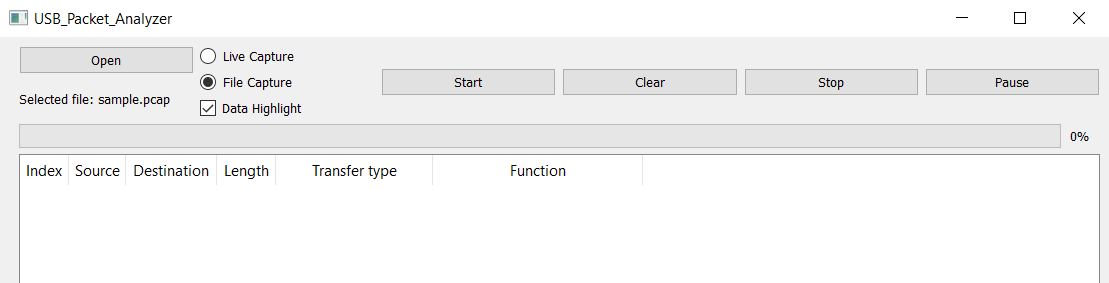
\includegraphics[width=\textwidth]{img/kap06_gui}
	\caption{Ukážka užívateľského rozhrania aplikácie.}
	\label{obr:kap6:gui}
\end{figure}

Teraz si postupne predstavíme jednotlivé tlačidlá:

\paragraph{Open} 
\hfill\break
Ako už samotný názov tlačidla napovedá, slúži na otváranie jednotlivých súborov, ktorých obsah budeme chcieť analyzovať.
Po jeho stlačení sa nám otvorí dialógové okno pomocou ktorého si zvolíme konkrétny pcap súbor. Akonáhle budeme mať daný súbor zvolený, pod tlačidlom bude vypísaný jeho názov.

\paragraph{Live Capture/File Capture}
\hfill\break
Nasleduje výber medzi Live Capture/File Capture pomocou RadioButtonov. File Capture reprezentuje analýzu ukončeného súboru, zatiaľ čo Live Capture podporuje analýzu súboru \uv{v reálnom čase}, takže je do súboru počas analýzy pripísať nové údaje, ktoré budú následne spracované aplikáciou.

\paragraph{Data Highlight}
Je CheckBox pomocou ktorého si užívateľ zvolí, či chce mať farebne zvýraznené položky v hexdumpe na základe ich významu alebo chce mať čistý hexdump bez farebného označenia. 

\paragraph{Start}
\hfill\break
Týmto tlačidlom spustíme analýzu zvoleného súboru. Ak sa navyše jedná o File Capture, progress bar pod tlačidlami nám percentuálne ukazuje akú časť súboru už máme spracovanú. Akonáhle progress bar dosiahne 100\%, celý súbor máme úspešne spracovaný a všetky základné informácie jednotlivých paketov (index, dĺžka, typ prenosu, atď.) sa zobrazia nižšie, pričom automaticky nás to posunie na úroveň posledného paketu. V prípade Live Capture to bude vyzerať podobne, ale progress bar nám momentálne nebude ukazovať percentuálnu časť spracovania súboru (pretože tá sa môže neustále meniť). Takisto nás to po odkončení analýzy posunie na úroveň aktuálneho paketu a to sa deje vždy keď sú do analýzy pridané nové pakety.

\paragraph{Clear}
\hfill\break
Toto tlačidlo nám vyčistí plochu do ktorej sú vyobrazované základné informácie jednotlivých paketov.

\paragraph{Stop}
\hfill\break
Toto tlačidlo je navrhnuté na používanie pri Live Capture kedy ukončí čítanie aktuálneho súboru a tým znemožní vyobrazenie nových paketov. Zároveň je tým znemožnená akákoľvek ďalšia analýza súborov. Toto tlačidlo užívateľ použije v prípade, že nemá záujem o analýzu nových paketov a stačia mu tie, ktoré má momentálne zobrazené v aplikácii.

\paragraph{Pause}
\hfill\break
Tlačidlo je tatiež navrhnuté na používanie pri Live Capture, kedy ním užívateľ dáva najavo, že chce pozastaviť pridávanie nových paketov na analýzu. Po jeho kliknutí sa nápis tlačidla zmení na \uv{Continue}, čím získava opačnú funkcionalitu -- obnovenie pridávania paketov. Všetky pakety, ktoré boli v súbore v intervale medzi stlačením Pause a Continue sú vynechané a pridávanie pokračuje od nasledujúcich paketov.



\section{Používanie aplikácie}
V tejto sekcii si ukážeme prácu s aplikáciou a ako vykonať File aj Live Capture analýzu. 

\subsection{Vytváranie pcap súborov}
Postup vytvárania súboru sa bude líšiť vzhľadom na to o aký druh analýzy máme záujem. Obecne je intuitívnejšie pracovať v oboch prípadoch s Wiresharkom ale v prípade, že si ho nechceme nainštalovať a máme záujem využívať iba možnosť File Capture, ukážeme si aj prácu s USBPcapom.

\subsubsection{File Capture}
Na vytvorenie pcap súboru pre File Capture máme na výber použiť USBPCap alebo Wireshark.

\paragraph{USBPcap}
Ak sa rozhodneme použiť USBPCap, postupujeme nasledovne:
\begin{enumerate}
\item Do tých USB portov, ktoré budeme chcieť počas zachytávania paketov sledovať pripojíme ľubovoľné HID zariadenie.
\item Zapneme USBPcap command line aplikáciu cez \textit{USBPcapCMD.exe}.
\item\label{kap6:sec:usbpcap_vyber_portov} Pomocou čísel si zvolíme USB porty, v ktorých máme zapojené zariadenia. Príklad vidíme na obrázku~\ref{obr:kap6:usbpcap_ports}, kde sú to porty 1 a 3.

\begin{figure}[!htb]
	\centering
	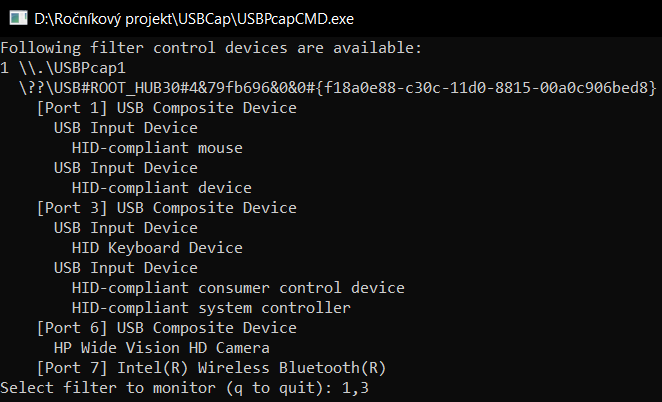
\includegraphics[width=12cm]{img/kap06_usbpcap_ports}
	\caption{Príklad vybratia portov 1 a 3 v aplikácii USBPcap.}
	\label{obr:kap6:usbpcap_ports}
\end{figure}

\item Následne si zvolíme meno súboru do ktrého chceme pakety zachytiť a stlačíme Enter. Vybehne nám \textit{Kontrola používateľských kont} v ktorej musíme povoliť USBPcap aplikácii vykonávanie zmien v zariadení. Predtým než to ale potvrdíme, odpojíme zariadenia zo všetkých USB portov, ktoré sme si zvolili vyššie. Toto robíme z dôvodu toho, aby sme už pri zachytávaní komunikácie dostali od zariadenia paket obsahujúci jeho HID Report Descriptor. V prípade, že zariadenia neodpojíme budeme mať síce zachytené všetky ostatné descriptory poslané počas konfigurácie, ale nebudeme schopní vykonať sémantickú analýzu inputu zariadení.
\item Po povolení vykonávaní zmien pripojíme do daných portov zariadenia, s ktorými chceme sledovať komunikáciu a môžeme s nimi vykonávať akcie, ktoré chceme mať zachytené.
\item Akonáhle chceme s analýzou skončiť, stlačíme klávesu \uv{q} a tým zároveň uončíme USBPCap. Momentálne by sme mali nájť náš súbor v priečinku v ktorom sa nachádza \textit{USBPcapCMD.exe}.
\end{enumerate}

USBPCap má ešte jednu nevýhodu -- zachytí konfiguráciu zariadení na všetkých USB portoch (aj tých, ktoré sme si v kroku~\ref{kap6:sec:usbpcap_vyber_portov} nezvolili). Samotnú komunikáciu s nimi už ale nesleduje.

\paragraph{Wireshark}
\label{kap6:sec:wireshark:file_capture}
V prípade použitia Wiresharku na vytváranie pcap sborov budeme nasledovať podľa týchto krokov:
\begin{enumerate}
\item Zapneme Wireshark aplikáciu cez \textit{Wireshark.exe}.
\item Upravíme nastavenia USBPCapu stlačením na sivé koliesko vedľa jeho názvu v oblasti \textit{Capture} dole (obrázok~\ref{obr:kap6:wireshark_usbpcap_settings}).

\begin{figure}[!htb]
	\centering
	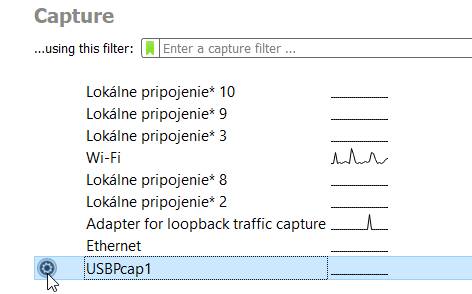
\includegraphics[width=10cm]{img/kap06_wireshark_usbpcap_settings}
	\caption{Ikona nastavenia USBPcapu vo Wiresharku.}
	\label{obr:kap6:wireshark_usbpcap_settings}
\end{figure}

\item Stlačíme tlačidlo \textit{Restore Defaults} a zašktrneme možnosť \textit{Capture from newly connected devices}. Bohužiaľ, pre uloženie týchto nastavení musíme spustiť jedno zachytávanie takže klikneme na tlačidlo \textit{Start} a potvrdíme \textit{Kontrolu používateľských kont}. Teraz môžeme toto zachytávanie zrušiť cez červený štvorec v hornej lište Wiresharku. Nastavenia sa nám týmto uložili a pokiaľ ich nebudeme chcieť zmeniť, nebudeme musieť tento krok už opakovať.
\item Teraz si vo Wiresharku cez možnosť \textit{Capture}$\rightarrow$\textit{Options} zaškrtneme v položke \textit{Input} možnosť USBPcap (obrázok~\ref{obr:kap6:wireshark_options_input}) a v položke \textit{Output} zvolíme možnosť \textit{pcap} a cez tlačidlo \textit{Browse} si vyberieme kde chceme uložiť súbor do ktorého budeme zachytávať komunikáciu (obrázok~\ref{obr:kap6:wireshark_options_output}).

\begin{figure}[!htb]
\centering
\begin{subfigure}{\textwidth}
  \centering
  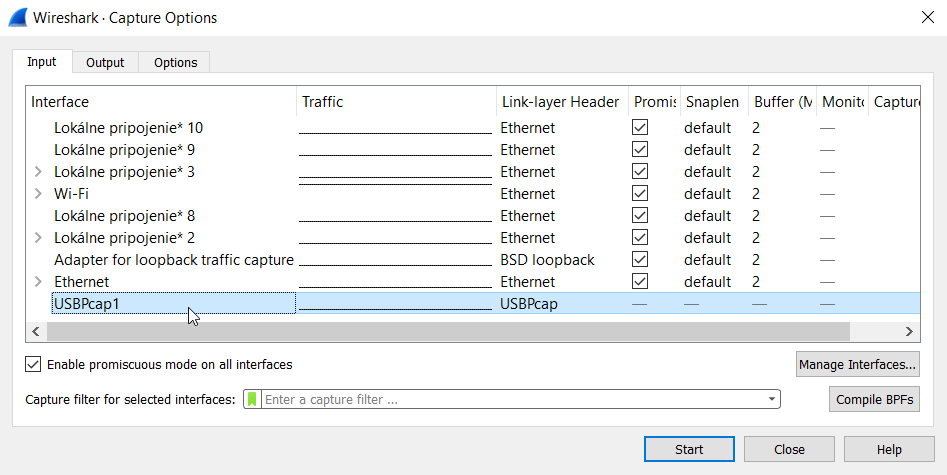
\includegraphics[width=\textwidth]{img/kap06_wireshark_options_input}
  \caption{Ukážka nastavenia inputu USBPcapu vo Wiresharku}
  \label{obr:kap6:wireshark_options_input}
\end{subfigure}
\begin{subfigure}{\textwidth}
  \centering
  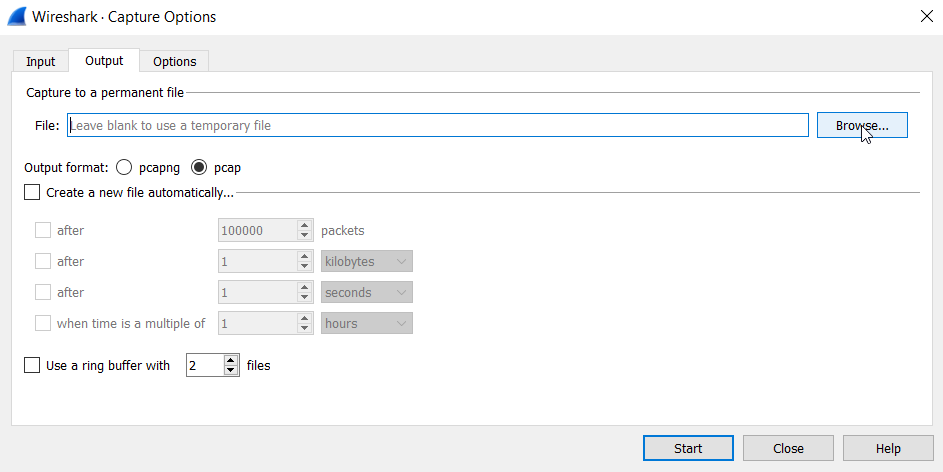
\includegraphics[width=\textwidth]{img/kap06_wireshark_options_output}
  \caption{Ukážka nastavenia outputu USBPcapu vo Wiresharku}
  \label{obr:kap6:wireshark_options_output}
\end{subfigure}
\caption{Ukážka nastavenia inputu a outputu USBPcapu vo Wiresharku}
\label{obr:kap6:wireshark_options_input_output}
\end{figure}

\item Skontrolujeme, že máme odpojené všetky zariadenia s ktorými chceme zachytávať komunikáciu a stlačíme tlačidlo \textit{Start}.
\item V momente keď budeme chcieť zachytávanie ukončiť, klikneme na červený štvorec v hornej lište Wiresharku.
\end{enumerate}

\subsubsection{Live Capture}
Na vykonanie Live Capture analýzy budeme potrebovať použiť aplikáciu Wireshark. Budeme postupovať pomocou rovnakých krokov ako pri File Capture~\ref{kap6:sec:wireshark:file_capture} s tou výnimkou, že teraz budeme mať počas zachytávania zapnutú aj našu aplikáciu ktorá bude vyobrazovať aktuálny stav súboru spolu s Wiresharkom.



\subsection{Príklad analýzy}
Momentálne si ukážeme konkrétny príklad File Capture analýzy na súbore \textit{sample.pcap}, ktorý je súčasťou prílohy k tejto práci. Budeme postupne zachytávať komunikáciu s 3 zariadeniami ukázanými na obrázku~\ref{obr:kap6:devices}:

\begin{figure}[!htb]
\centering
\begin{subfigure}{.4\textwidth}
  \centering
  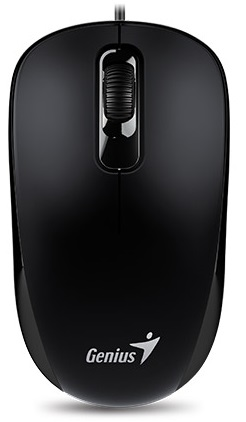
\includegraphics[width=.4\linewidth]{img/genius_mys.jpg}
  \caption{Fotka genius myši prevzatá z oficiálnej genius stránky~\cite{genius_mouse_pic}.}
  \label{obr:kap6:genius:mouse:pic}
\end{subfigure}%
\begin{subfigure}{.6\textwidth}
  \centering
  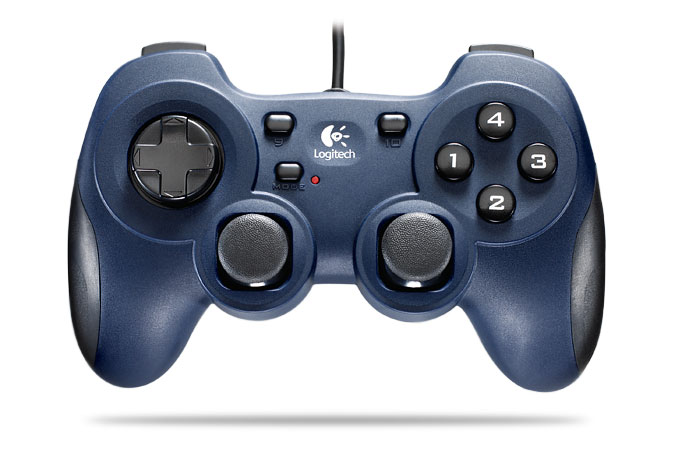
\includegraphics[width=.6\linewidth]{img/kap06_joystick}
  \caption{Fotka logitech joysticku prevzatá zo stránky obchodu~\cite{logitech_joystick_pic}.}
  \label{obr:kap6:joystick_obr}
\end{subfigure}
\begin{subfigure}{\textwidth}
  \centering
  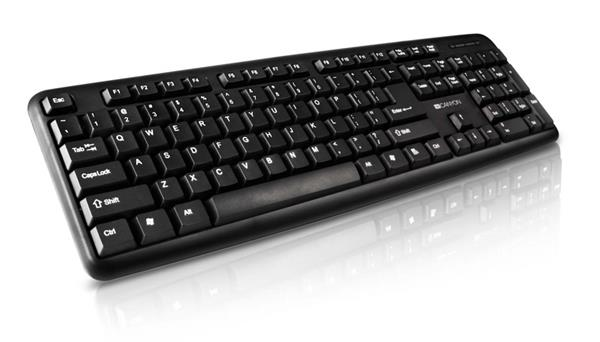
\includegraphics[width=\textwidth]{img/kap06_keyboard}
  \caption{Fotka CANYON klávesnice prevzatá zo stránky obchodu~\cite{canyon_keyboard_pic}.}
  \label{obr:kap6:keyboard_obr}
\end{subfigure}
\caption{Ukážka zariadení s ktorými budeme zachytávať komunikáciu.}
\label{obr:kap6:devices}
\end{figure}


Počas zachytávania sme vykonali nasledujúce:
\begin{enumerate}
\item Do USB portu sme pripojili zariadenie myši.
\item Stlačili sme ľavé tlačidlo myši.
\item Stlačili sme pravé tlačidlo myši.
\item Posunuli sme koliekom myši smerom dole.
\item Vykonali sme pohyb s myšou a naásledne ju odpojili.
\item Pripojili sme zariadenie klávesnice.
\item Stlačili a pustili sme tlačidlo \uv{A}.
\item Stlačili a podržali sme tlačidlo \uv{C} a potom tlačidlo \uv{D}, následne sme pustili tlačidlo \uv{C} a potom \uv{D}.
\item Stlačili a pustili sme tlačidlo \uv{Tab}.
\item Do druhého USB portu sme pripojili zariadenie joysticku.
\item Na joysticku sme stlačili s pustili sme tlačidlo \uv{1} a následne tlačidlo \uv{8}.
\item Stlačili a pustili sme niekoľko tlačidiel naraz.
\item Vykonali sme pohyb analógom.
\item Ukončili sme zachytávanie.
\end{enumerate}

Teraz si otvoríme našu aplikáciu, pomocou tlačilda \uv{Open} si vyberieme súbor s vyššie opísanou zachytenou komunikáciou a stlačíme tlačidlo \uv{Start}. Pre bližšiu analýzu jednotlivých paketov dvojklikneme na riadok, ktorý daný paket reprezentuje. To má za následok vytvorenie pop-up okna (obrázok~\ref{obr:kap6:uk_popup}), ktoré má nasledujúce rozloženie:
\begin{itemize}
\item Vľavo hore máme vyobrazenú stromovú štruktúru, ktorá detailnejšie opisuje hlavičku paketu.
\item Vpravo hore je vyobrazená stromová štruktúra reprezentujúca sémantický význam zyvškových dát paketu.
\item Vľavo dole máme stromovú štruktúru opisujúcu farby v Color Map pre jenoduchšiu orientáciu v hexdumpe.
\item Vedľa Color Map sa nachádza daný hexdump, pričom tabuľka vľavo vyobrazuje znaky v ich hexadecimálnej podobe a tabuľka vpravo vyobrazuje dané znaky v ich tlačiteľnej podobe.
\end{itemize}

\begin{figure}[!htb]
	\centering
	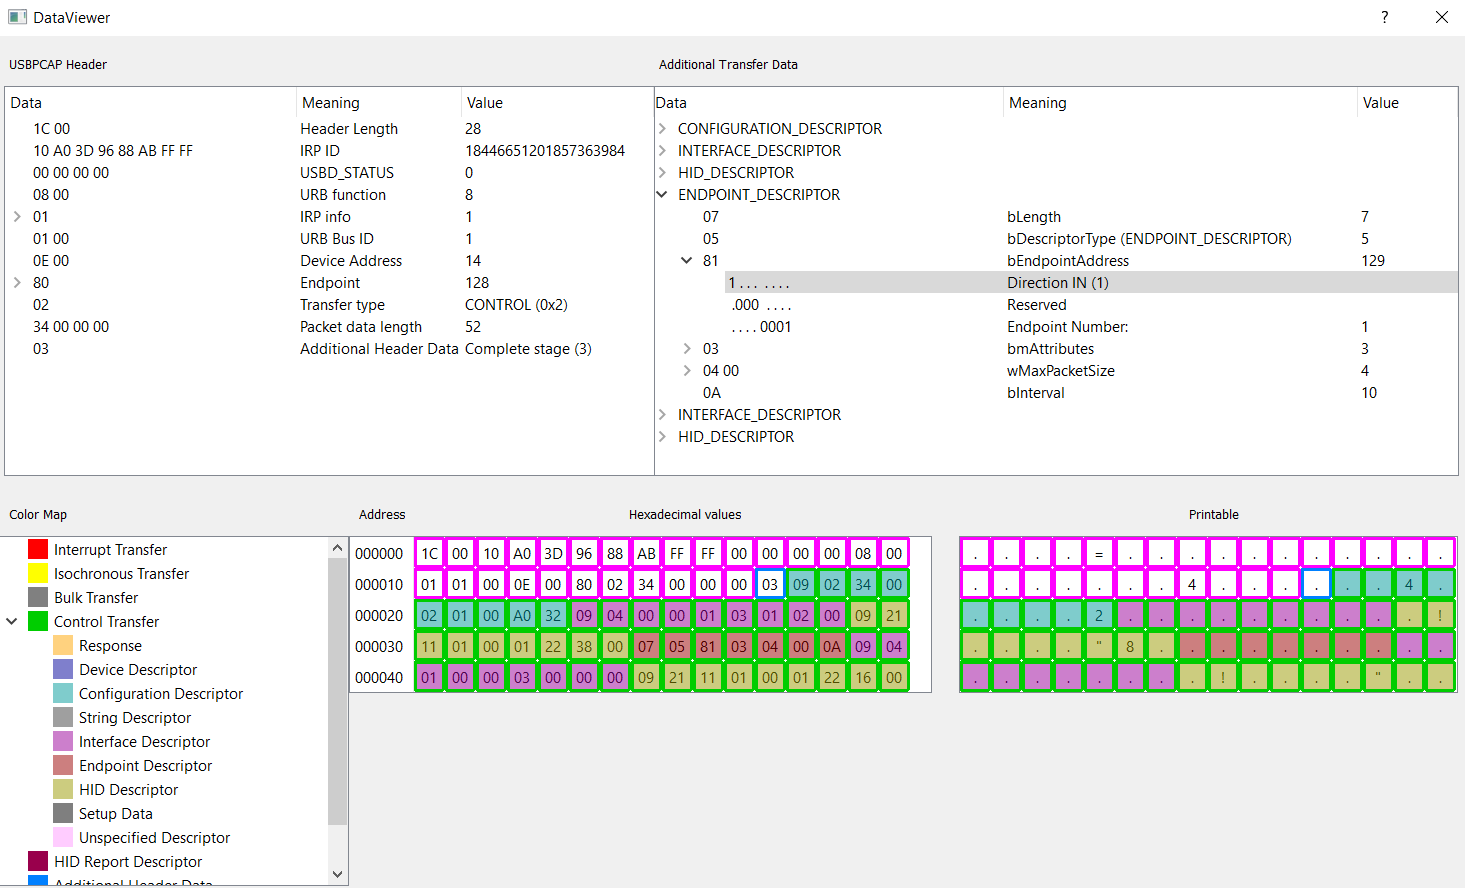
\includegraphics[width=\textwidth]{img/kap06_uk_popup}
	\caption{Ukážka užívateľského rozhrania aplikácie.}
	\label{obr:kap6:uk_popup}
\end{figure}

Momentálne si už len ukážeme zopár obrázkov analýzy vyššie spomínanej komunikácie.

\begin{figure}[!htb]
	\centering
	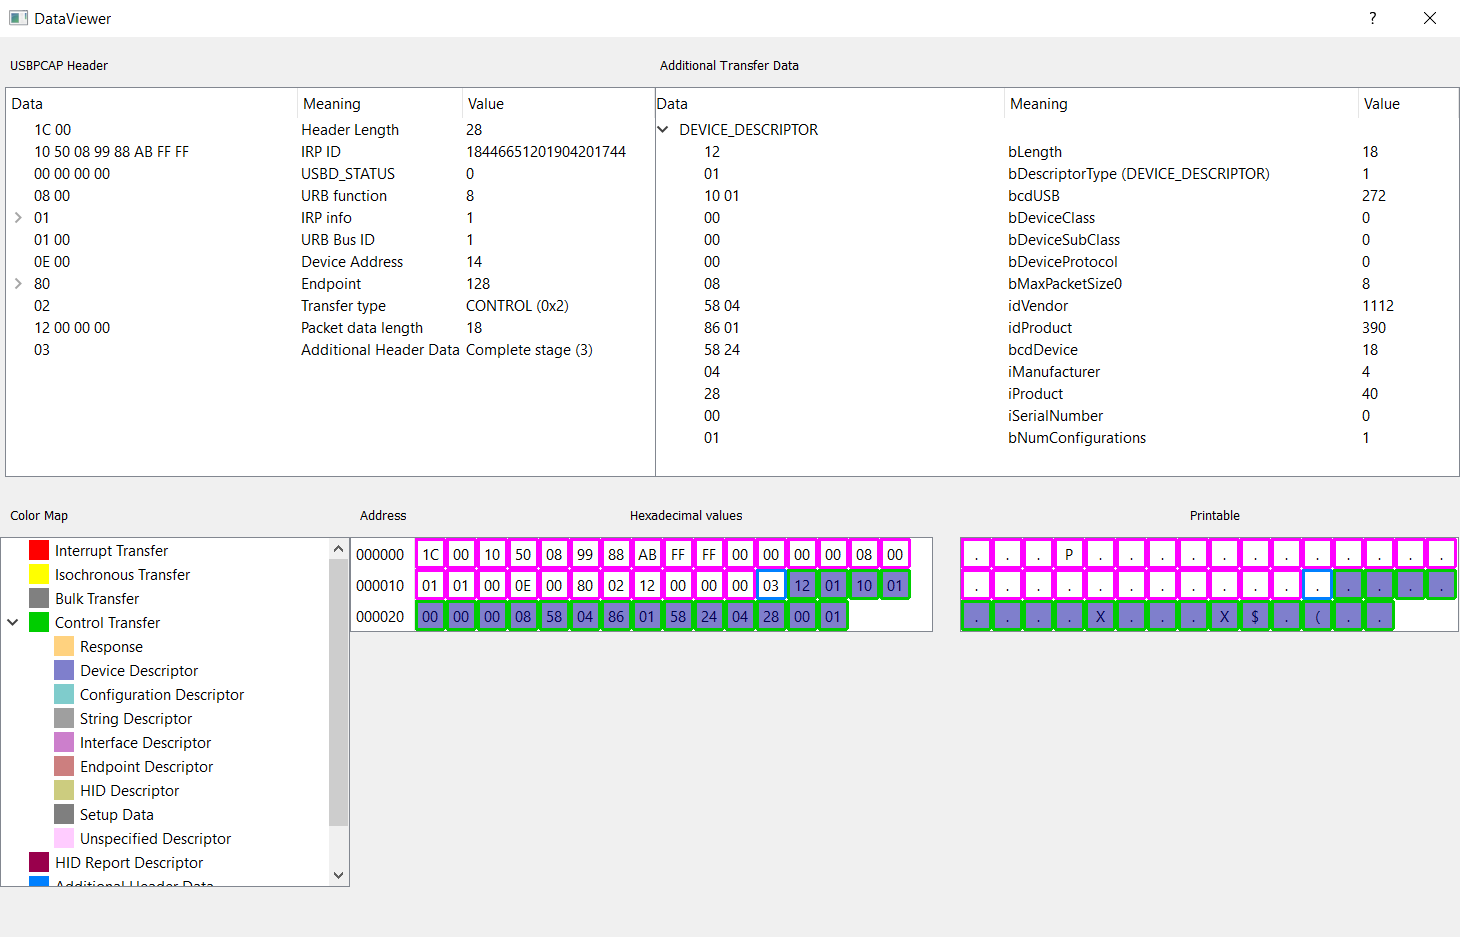
\includegraphics[width=\textwidth]{img/kap06_device_desc}
	\caption{Ukážka Device Descriptoru myši.}
	\label{obr:kap6:uk_device_desc}
\end{figure}

\begin{figure}[!htb]
	\centering
	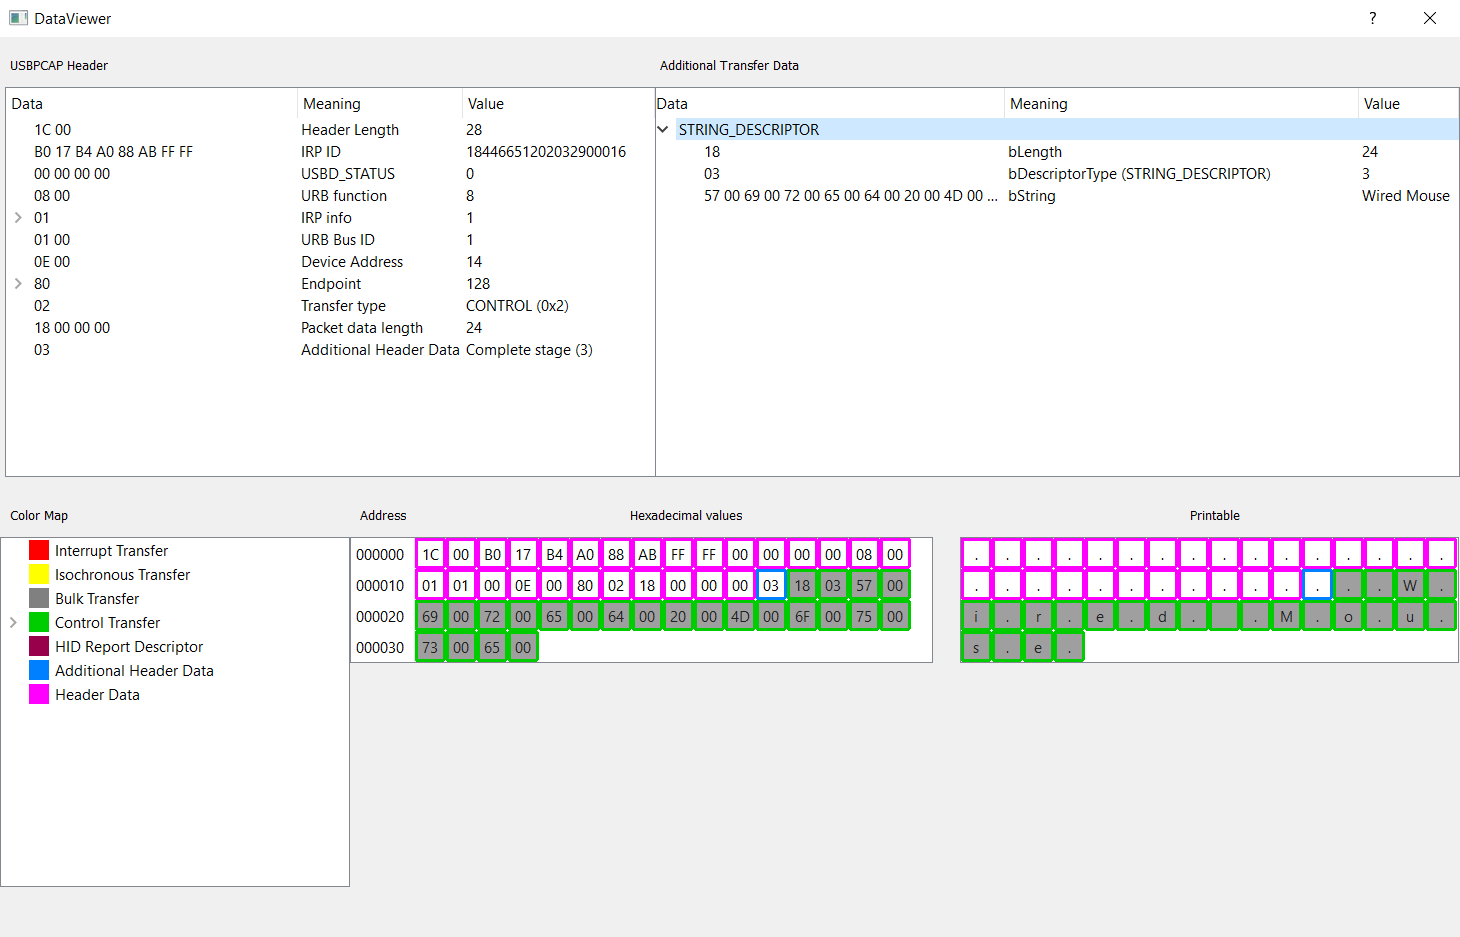
\includegraphics[width=\textwidth]{img/kap06_uk_string_descriptor}
	\caption{Ukážka String Descriptoru myši.}
	\label{obr:kap6:uk_string_desc}
\end{figure}

\begin{figure}[!htb]
	\centering
	\includegraphics[width=\textwidth]{img/kap06_uk_report_desc}
	\caption{Ukážka Report Descriptoru joysticku.}
	\label{obr:kap6:uk_report_desc}
\end{figure}

\begin{figure}[!htb]
	\centering
	\includegraphics[width=\textwidth]{img/kap06_uk_mouse}
	\caption{Ukážka inputu myši.}
	\label{obr:kap6:uk_input_mouse}
\end{figure}

\begin{figure}[!htb]
	\centering
	\includegraphics[width=\textwidth]{img/kap06_uk_keyboard}
	\caption{Ukážka inputu klávesnice.}
	\label{obr:kap6:uk_input_keyboard}
\end{figure}

\begin{figure}[!htb]
	\centering
	\includegraphics[width=\textwidth]{img/kap06_uk_joystick}
	\caption{Ukážka inputu joysticku.}
	\label{obr:kap6:uk_input_joystick}
\end{figure}









































\chapter{Záver}
\section{Zhrnutie}
celkove zhrnutie prace, ?praca s Qt?
\section{Budúce plány}




%%% Seznam použité literatury
%%% Seznam použité literatury (bibliografie)
%%%
%%% Pro vytváření bibliografie používáme bibTeX. Ten zpracovává
%%% citace v textu (např. makro \cite{...}) a vyhledává k nim literaturu
%%% v souboru literatura.bib.
%%%
%%% Příkaz \bibliographystyle určuje, jakým stylem budou citovány odkazy
%%% v textu. V závorce je název zvoleného souboru .bst. Styly plainnat
%%% a unsrt jsou standardní součástí latexových distribucí. Styl czplainnat
%%% je dodáván s touto šablonou a bibTeX ho hledá v aktuálním adresáři.

% \bibliographystyle{czplainnat}    %% Autor (rok) s českými spojkami
% \bibliographystyle{plainnat}    %% Autor (rok) s anglickými spojkami
\bibliographystyle{unsrt}       %% [číslo]

\renewcommand{\bibname}{Zoznam použitej literatúry}

%%% Vytvoření seznamu literatury. Pozor, pokud jste necitovali ani jednu
%%% položku, seznam se automaticky vynechá.

\bibliography{outro/literatura}

%%% Kdybyste chtěli bibliografii vytvářet ručně (bez bibTeXu), lze to udělat
%%% následovně. V takovém případě se řiďte normou ISO 690 a zvyklostmi v oboru.

% \begin{thebibliography}{99}
%
% \bibitem{lamport94}
%   {\sc Lamport,} Leslie.
%   \emph{\LaTeX: A Document Preparation System}.
%   2. vydání.
%   Massachusetts: Addison Wesley, 1994.
%   ISBN 0-201-52983-1.
%
% \end{thebibliography}


%%% Obrázky v bakalářské práci
%%% (pokud jich je malé množství, obvykle není třeba seznam uvádět)
\listoffigures

%%% Tabulky v bakalářské práci (opět nemusí být nutné uvádět)
%%% U matematických prací může být lepší přemístit seznam tabulek na začátek práce.
%\listoftables

%%% Použité zkratky v bakalářské práci (opět nemusí být nutné uvádět)
%%% U matematických prací může být lepší přemístit seznam zkratek na začátek práce.
%\chapwithtoc{Seznam použitých zkratek}

%%% Přílohy k bakalářské práci, existují-li. Každá příloha musí být alespoň jednou
%%% odkazována z vlastního textu práce. Přílohy se číslují.
%%%
%%% Do tištěné verze se spíše hodí přílohy, které lze číst a prohlížet (dodatečné
%%% tabulky a grafy, různé textové doplňky, ukázky výstupů z počítačových programů,
%%% apod.). Do elektronické verze se hodí přílohy, které budou spíše používány
%%% v elektronické podobě než čteny (zdrojové kódy programů, datové soubory,
%%% interaktivní grafy apod.). Elektronické přílohy se nahrávají do SISu a lze
%%% je také do práce vložit na CD/DVD. Povolené formáty souborů specifikuje
%%% opatření rektora č. 72/2017.
\appendix
%%% Přílohy k bakalářské práci, existují-li. Každá příloha musí být alespoň jednou
%%% odkazována z vlastního textu práce. Přílohy se číslují.
%%%
%%% Do tištěné verze se spíše hodí přílohy, které lze číst a prohlížet (dodatečné
%%% tabulky a grafy, různé textové doplňky, ukázky výstupů z počítačových programů,
%%% apod.). Do elektronické verze se hodí přílohy, které budou spíše používány
%%% v elektronické podobě než čteny (zdrojové kódy programů, datové soubory,
%%% interaktivní grafy apod.). Elektronické přílohy se nahrávají do SISu a lze
%%% je také do práce vložit na CD/DVD. Povolené formáty souborů specifikuje
%%% opatření rektora č. 72/2017.

\chapwithtoc{Prílohy}

%section{První příloha}

\openright
\end{document}
